% Copyright (c) 2022 Ludovic Lars
% This work is licensed under the CC BY-NC-SA 4.0 International License

\chapter{La détermination du protocole}
\label{ch:determination}

Une monnaie est un accord concernant un moyen mutuellement acceptable dans le commerce. Cet accord peut porter sur des propriétés physiques, auquel cas le support monétaire est une marchandise, ou des propriétés numériques, auquel cas le support monétaire est un protocole informatique. Bitcoin appartient à cette seconde catégorie.

De par sa nature ouverte et libre, le code informatique de Bitcoin peut être copié, modifié et réutilisé à volonté. Par conséquent, le protocole peut lui aussi être modifié et multiplié. Bitcoin n'est pas un système figé et unique qui serait géré par une autorité centrale, mais un modèle ouvert qui connaît une évolution organique et plurielle au cours du temps.

Cette évolution est un mécanisme économique, conformément à la nature essentiellement monétaire de Bitcoin. Les règles qui garantissent le bon fonctionnement du système résultent donc du choix réalisé par les agents économiques. En particulier, la résistance à l'inflation, ou la difficulté à créer plus de bitcoins, n'émerge pas de l'établissement de la politique monétaire arbitraire par Satoshi Nakamoto, mais de la dynamique économique opposée à l'altération de cette politique monétaire.

\section*{La résistance à l'inflation}
\addcontentsline{toc}{section}{La résistance à l'inflation}

% Propriété de résistance à l'inflation
L'une des deux grandes promesses de Bitcoin est de résister à l'inflation monétaire, c'est-à-dire de rendre difficile la création supplémentaire d'unités par rapport à ce qui est accepté par le marché. Cette promesse est énorme~: comme on l'a vu dans le chapitre~\ref{ch:adversaire}, l'État fait tout ce qu'il peut pour profiter de la création monétaire, phénomène qu'on appelle le seigneuriage. De prime abord, il paraît ainsi étonnant qu'un objet numérique puisse posséder une telle propriété.

% Politique monétaire
La politique monétaire classique du bitcoin a été établie par Satoshi Nakamoto lors du lancement du prototype le 8 janvier 2009\sendnote{Satoshi Nakamoto, \eng{Bitcoin v0.1 released}, \wtime{08/01/2009 19:27:40 UTC}~: \url{https://www.metzdowd.com/pipermail/cryptography/2009-January/014994.html}.}. Celle-ci possédait un caractère simple~: la création monétaire devait être réduite de moitié tous les quatre ans, de façon à devenir négligeable au bout d'un temps. Il devait se créer 10,5 millions d'unités de manière linéaire les quatre premières années, 5,25 millions les quatre suivantes, 2,625 millions les quatre d'après, et ainsi de suite, ce qui limitait le nombre d'unités en circulation à 21 millions. Le bitcoin devait finir par devenir une monnaie à quantité fixe, quelque chose n'ayant jamais été vu dans l'histoire\sendnote{Voir chapitre~\ref{ch:origine}, section «~Une nouvelle forme de monnaie~».}.

% Aspect mathématique
Cette politique monétaire a été l'un des arguments de vente de Bitcoin, si bien que certaines personnes se sont imaginées qu'il s'agissait de quelque chose d'immuable, de gravé dans le marbre et que l'application mathématique de ce décret de Satoshi Nakamoto était ce qui garantissait la résistance à l'inflation du système. On l'a par exemple vu avec Tyler Winklevoss qui se convainquait en 2013 qu'il avait acheté un actif dépourvu d'intervention humaine~:

\begin{quote}
«~Nous avons choisi de placer notre argent et notre confiance dans un cadre mathématique exempt de politique et d'erreur humaine.\sendnote{Nathaniel Popper et Peter Lattman, \eng{As Big Investors Emerge, Bitcoin Gets Ready for its Close-Up}, 11 avril 2013~: \url{https://www.cnbc.com/id/100635418}.}~»
\end{quote} % We have elected to put our money and faith in a mathematical framework that is free of politics and human error.

Toutefois, cette conception est au mieux une approximation maladroite. Il ne suffit pas que qu'une règle ait été décrétée par quelqu'un dans le passé pour qu'elle se manifeste dans la réalité, il faut aussi que d'autres personnes l'acceptent et l'appliquent. Et cette acceptation est précisément soumise à la politique et à l'erreur humaine.

% Question de la gouvernance
Il existe au sujet de la politique monétaire fixe du bitcoin une certaine confusion. Il faut dire que Satoshi Nakamoto n'a jamais explicité comment elle pouvait être protégée. Plusieurs théories ont été proposées, allant de l'intervention des mineurs à l'exigence d'unanimité communautaire\sendnote{River Financial, \eng{Can Bitcoin's Hard Cap of 21 Million Be Changed?}~: \url{https://river.com/learn/can-bitcoins-hard-cap-of-21-million-be-changed}.}, en passant par le caractère juridique du décret\sendnote{\url{https://craigwright.net/blog/law-regulation/forking-and-passing-off/}}. Dans tous les cas, il s'agissait de traiter la question de la gouvernance\sendnote{Pierre Rochard, \eng{Bitcoin Governance}, 9 juillet 2018~: \url{https://pierre-rochard.medium.com/bitcoin-governance-37e86299470f}.} ou du consensus social\sendnote{Arthur Breitman parlait de \eng{social consensus} dès août 2014 dans la première description formelle de Tezos. -- Arthur Breitman, \eng{Tezos: A Self-Amending Crypto-Ledger}, 3 août 2014~: \url{https://tezos.com/position-paper.pdf}.}, c'est-à-dire de la façon dont les règles sont décidées dans Bitcoin. Cette problématique, nous l'appelons ici la détermination du protocole.

\section*{Le protocole}
\addcontentsline{toc}{section}{Le protocole}

% Nature protocolaire de Bitcoin
Bitcoin est par essence un protocole de communication informatique, c'est-à-dire un ensemble de règles permettant à différentes parties d'un réseau d'échanger des informations. Ce protocole permet aux nœuds du réseau pair-à-pair de s'échanger des transactions et des blocs et de se mettre d'accord sur le registre de propriété à considérer comme correct. Il crée par conséquent un système monétaire.

% Autres protocoles liés à Internet
Bitcoin se rapproche, de façon plus ou moins de protocoles existants. C'est par exemple le cas d'autres protocoles construits sur Internet, comme HTTP (\eng{HyperText Transfer Protocol}) qui est utilisé pour l'affichage des pages web, SMTP (\emph{Simple Mail Transfer Protocol}) qui est utilisé pour le courrier électronique, ou encore BitTorrent, qui permet le partage de fichiers de pair à pair. C'est également le cas des protocoles qui soutiennent Internet, appelés protocoles de la suite TCP/IP en référence aux deux premiers qui la composent~: IP (\eng{Internet Protocol}) qui assure la communication au niveau de la couche réseau, et TCP (\eng{Transmission Control Protocol}) qui assure la transmission au niveau de la couche transport, en surcouche de la couche réseau.

% Langages de programmation et langues
Plus éloigné de Bitcoin, on peut citer la catégorie des langages de programmation. Ces langages permettent d'écrire du code (texte spécifique encodé en UTF-8), qui est transformé en fichier exécutable par un compilateur (comme dans le cas du C, du C++ ou du Java) ou qui est directement exécuté par un interpréteur (comme dans le cas du Python ou du Javascript). Dans le même ordre d'idées, les langues humaines comme le français ou l'anglais sont aussi des protocoles de communication, dont les règles sont moins formelles et moins bien définies, mais qui permet aux hommes d'échanger des informations.

% Monnaies
Enfin, les monnaies peuvent être vues comme des sortes de protocole, en constituant des moyens communs de communiquer de la valeur et de formaliser l'échange économique. La monnaie se définit en particulier par le support accepté dans le commerce~: pour une marchandise comme l'or ou l'argent, ce support est un élément chimique~; pour la monnaie fiat, il s'agit d'un certificat émis par une autorité.

% Bitcoin : deux sous-protocoles
Dans le cas de Bitcoin, le protocole est formé de l'ensemble des règles qui permettent au réseau de communiquer et de se coordonner. Ce protocole se divise en deux parties distinctes~: le protocole de transmission, constitué des règles de réseau, et le protocole régissant le contenu transmis, constitué des règles de consensus.

% Règles de réseau
Les règles de réseau sont les règles qui permettent aux nœuds d'entrer en communication sur Internet. Ces règles concernent le protocole de transport sous-jacent (TCP, Tor, UDP pour FIBRE), le port réseau (8333 pour le réseau principal BTC), la procédure de découverte de pairs, la syntaxe des messages de transmission de données\sendnote{\url{https://en.bitcoin.it/wiki/Protocol_documentation\#Common\_structures}},~etc. Elles peuvent différer selon les nœuds sans briser formellement le consensus~: il suffit qu'un nœud acceptant les deux ensembles de règles fasse la liaison. De même, les nœuds sont libres de restreindre (temporairement ou définitivement) leur connexion avec un autre nœud, notamment dans le but d'éviter le spam.

% Règles de consensus
Les règles de consensus sont les règles de construction et d'organisation des blocs et des transactions. Elles régissent donc la validité du registre sur lequel les membres du réseau arrivent à un accord. Ces règles sont critiques~: un nœud qui transmettrait une transaction ou un bloc invalide aux autres nœuds verrait sa transaction ou son bloc être rejeté par le reste du réseau.

% Exemples
Les règles de consensus sont nombreuses. Certaines d'entre elles sont largement connues et explicites. En voici quelques-unes ici~:

\begin{itemize}
\item[$\bullet$] Le montant en entrée d'une transaction doit être supérieur (ou égal) au montant en sortie, la différence représentant les frais collectés par le mineur~;
\item[$\bullet$] Chaque entrée doit contenir un script de déverrouillage (contenant la ou les signatures) qui correspond au script de verrouillage (l'adresse d'envoi) de la sortie dépensée~;
\item[$\bullet$] Une sortie transactionnelle ne peut être dépensée qu'une seule fois, en raison de l'interdiction de double dépense~;
\item[$\bullet$] Chaque bloc doit comporter une preuve de travail, produite par hachages répétés de l'entête par la fonction SHA-256, de degré supérieur à la difficulté du réseau~;
\item[$\bullet$] La subvention dans chaque bloc doit être inférieure à une limite, qui est divisée par deux tous les 210~000 blocs (4 ans environ)~;
\item[$\bullet$] La difficulté du minage est ajustée tous les 2016 blocs (2 semaines environ), de sorte à garantir un temps moyen de 10 minutes entre chaque bloc~;
\item[$\bullet$] Le poids des blocs est limité à 4 millions d'unités de poids (telles que définies par SegWit), ce qui restreint la capacité transactionnelle du système.
\end{itemize}

Les règles de consensus sont trop nombreuses pour être toutes explicitées. Quand elles ne le sont pas, ces règles sont implicitement définies dans l'implémentation logicielle de référence, qui est Bitcoin Core dans le cas de BTC.

\section*{Les implémentations logicielles}
\addcontentsline{toc}{section}{Les implémentations logicielles}

% --- Les implémentations logicielles ---

% Implémentations complètes et partielles
Les implémentations logicielles sont les programmes informatiques qui mettent en œuvre le protocole. Dans le cas des implémentations de nœud complet, l'ensemble des règles de consensus sont appliquées. Les implémentations peuvent également être partielles, auquel cas elles ne mettent pas en œuvre pas l'intégralité des règles de consensus~: c'est par exemple le cas des portefeuilles, qui procèdent à une vérification simplifiée de leurs transactions.

% Implémentations dans BTC
Dans BTC, il existe plusieurs implémentations, dont Bitcoin Core, Libbitcoin, btcd et Bitcoin Knots. La plus connue est Bitcoin Core, qui est à la fois l'implémentation historique créée par Satoshi Nakamoto («~\eng{Satoshi client}~») et reprise par Gavin Andresen en 2010, l'implémentation principale utilisée par \textcolor{darkgray}{plus de 98~\% des nœuds en avril 2023}\sendnote{\url{https://coin.dance/nodes}}, et l'implémentation de référence, qui définit les règles de consensus implicites.

% Implémentations dans BCH et ETH
D'autres protocoles possèdent des implémentations différentes. Bitcoin Cash possède une multiplicité d'implémentations~: Bitcoin Cash Node (l'implémentation de référence issu de Bitcoin ABC issu de Bitcoin Core), Bitcoin Unlimited, bchd et Bitcoin Verde. Ethereum possède également une diversité d'implémentations\sendnote{\url{https://clientdiversity.org/\#distribution}}, qui gèrent la transmission et la vérification des transactions (Geth, Nethermind, etc.) ou celles des blocs (Prysm, Lighthouse, etc.)

% Logiciel libre
Une implémentation est en règle générale un logiciel libre, c'est-à-dire un logiciel dont le code est publié en accès libre sous une licence permettant l'utilisation, la modification et la reproduction. Cette caractéristique, technique et juridique, est \emph{essentielle} à Bitcoin, car elle permet non seulement de vérifier le fonctionnement du logiciel\sendnote{«~L'accès en source ouverte signifie que n'importe qui peut examiner le code de manière indépendante. S'il s'agissait d'une source fermée, personne ne pourrait vérifier la sécurité. Je pense qu'il est essentiel pour un programme de cette nature d'être en source ouverte. -- Satoshi Nakamoto, \eng{Re: Questions about Bitcoin}, \wtime{10/12/2009 20:49:02 UTC}~: \url{https://bitcointalk.org/index.php?topic=13.msg46\#msg46}.}, mais aussi de reprendre la main sur le code dans le cas où les développeurs iraient dans une direction non désirée.

% Fork
L'action de copier et de modifier un logiciel est appelé un \eng{fork} ou embranchement. Il s'agit de créer un nouveau logiciel à partir du code source d'un logiciel existant, dont l'existence découle d'une vision différente du développement de ce logiciel. Les distributions Linux sont ainsi formées de distributions antérieures\sendnote{\url{https://upload.wikimedia.org/wikipedia/commons/9/96/Liste_des_distributions_Linux.svg}}. On peut aussi citer OpenOffice.org qui a donné LibreOffice et Apache OpenOffice.

% Historique de Bitcoin Core
Bitcoin Core descend directement de la première implémentation codée par Satoshi Nakamoto et partagée publiquement le 8 janvier 2009. Initialement appelé simplement «~Bitcoin~», le logiciel a été renommé en bitcoind~/~Bitcoin-Qt en 2011, puis en Bitcoin Core le 19 mars 2014\sendnote{\eng{Bitcoin Core version 0.9.0 released}, 19 mars 2014~: \url{https://bitcoin.org/en/release/v0.9.0\#rebranding-to-bitcoin-core}.}.

% Code source
Bitcoin Core est un logiciel codé en C++. Initialement hébergé sur SourceForge, il est aujourd'hui présent sur GitHub\sendnote{\eng{Bitcoin Core integration/staging tree}~: \url{https://github.com/bitcoin/bitcoin}.}. Le code est publié sous licence libre MIT, de sorte que quiconque peut le copier et le modifier à sa guise. En particulier, la licence MIT est permissive~: elle n'empêche pas la réutilisation du code comme partie ou comme base d'un logiciel soumis à une licence privative. Cette licence a été choisie par Satoshi au détriment de la licence GPL en raison de sa compatibilité avec les autres licences\sendnote{Satoshi Nakamoto, \eng{Re: Switch to GPL}, \wtime{12/09/2010 19:24:53 UTC}~: \url{https://bitcointalk.org/index.php?topic=989.msg12494\#msg12494}.}.

% Développement de Bitcoin Core
Le développement de Bitcoin Core se fait de manière ouverte et méritocratique. Le dépôt GitHub est ouvert à tous et n'importe qui peut contribuer au développement en faisant une demande de modification du code (\eng{pull request}). Les contributeurs fréquents sont appelés des «~\eng{core developers}~». Pour faciliter le développement, les contributeurs communiquent par différents moyens, mais les deux principaux sont le canal IRC bitcoin-core-dev où ont lieu la plupart des discussions et la liste de diffusion bitcoin-dev\sendnote{The bitcoin-dev Archives~: \url{https://lists.linuxfoundation.org/pipermail/bitcoin-dev/}}.

% Hiérarchie
Toutefois, Bitcoin Core dispose d'une certaine hiérarchie. Ainsi le dépôt est géré par des mainteneurs qui sont responsables de fusionner les demandes de modification créées par les contributeurs. L'inclusion dans le code dépend ainsi de différents critères évalués par ces mainteneurs, comme l'utilité démontrable du changement, le format correct suivant les lignes directrices du projet, la revue par les pairs ou la réputation du contributeur\sendnote{«~Les mainteneurs prendront en considération un correctif s'il est en accord avec les principes généraux du projet~; s'il répond aux normes minimales d'inclusion~; et jugeront du consensus général des contributeurs.~» -- \eng{Contributing to Bitcoin Core}, 2023~: \url{https://github.com/bitcoin/bitcoin/blob/25.x/CONTRIBUTING.md}.}. % Maintainers will take into consideration if a patch is in line with the general principles of the project; meets the minimum standards for inclusion; and will judge the general consensus of contributors.

% Mainteneur principal
La charge du logiciel était initialement allouée à un mainteneur principal, qui avait pour rôle de nommer les mainteneurs, de décider du cycle de sortie du logiciel, de fusionner l'ensemble des modifications et de modérer les débats. Cette mission était assurée au début par Satoshi Nakamoto qui s'occupait d'intégrer les contributions sur le dépôt SourceForge. Puis, le 23 février 2011, Satoshi a transmis la responsabilité à Gavin Andresen, avant de disparaître définitivement. Gavin s'est ensuite chargé du projet pendant plus de trois ans avant de laisser sa place à Wladimir J. van der Laan le 7 avril 2014. Enfin, le 7 février 2023, ce dernier a démissionné après neuf ans de service, et la fonction de mainteneur principal a été supprimée et remplacée par la responsabilité collective des mainteneurs\sendnote{Wladimir J. van der Laan, \eng{The widening gyre}, 21 janvier 2021~: \url{https://laanwj.github.io/2021/01/21/decentralize.html}~, archive~: \url{https://web.archive.org/web/20210121201607/https://laanwj.github.io/2021/01/21/decentralize.html}~; Wladimir J. van der Laan, \eng{Remove laanwj from trusted-keys (git commit)}, \wtime{07/02/2023 09:12 UTC}~: \url{https://github.com/bitcoin/bitcoin/commit/aafa5e945cef7a4f65ddadcf548932dd4e27ada1}.}.

% Mainteneurs
\textcolor{darkgray}{En juin 2023}, les mainteneurs de Bitcoin Core étaient au nombre de cinq~: Michael Ford, Hennadii Stepanov, Andrew Chow, Gloria Zhao et Ryan Ofsky. Ils suivent la voie de mainteneurs emblématiques (hors mainteneurs principaux) comme Martti Malmi, Laszlo Hanyecz, Chris Moore, Pieter Wuille, Jeff Garzik, Nils Schneider, Gregory Maxwell, Jonas Schnelli, Samuel Dobson ou Marco Falke\sendnote{Andrew Chow, \eng{List of people who have had commit access to Bitcoin Core}, \wtime{07/07/2022 20:05:39 UTC}~: \url{https://bitcointalk.org/index.php?topic=1774750.msg17700787\#msg17700787}.}. Parmi les contributeurs actifs qui n'ont jamais été mainteneurs, on retrouve Matt Corallo, practicalswift, luke-jr et John Newbery.  Les empreintes PGP des mainteneurs sont disponibles publiquement sur le dépôt.

% Solidité du logiciel
Ce fonctionnement ouvert donne au logiciel une sûreté plus grande que la plupart des programmes informatiques. En effet, au vu des sommes en jeu, la récompense pour l'exploitation réussie d'une faille majeure serait énorme, si bien qu'on peut supposer qu'une telle faille n'a pas été découverte. S'il y a effectivement des vulnérabilités dans le logiciel, celles-ci sont très rares et très subtiles, de sorte qu'elles sont généralement découvertes par des développeurs bienveillants, à l'instar du développeur Awemany qui avait, en septembre 2018, divulgué de manière responsable une faille inflationniste dans le code\sendnote{Awemany, \eng{600 Microseconds}, 21 septembre 2018~: \url{https://medium.com/@awemany/600-microseconds-b70f87b0b2a6}.}. Ainsi, le passage du temps renforce la confiance qu'on peut avoir dans le logiciel (ainsi que dans le système) conformément à l'effet Lindy\sendnote{«~Chaque jour qui passe sans que Bitcoin ne s'effondre en raison de problèmes juridiques ou techniques apporte de nouvelles informations au marché. Cela augmente les chances de succès de Bitcoin et justifie un prix plus élevé.~» -- Hal Finney, \eng{Re: Bitcoin and the Efficient Market Hypothesis}, \wtime{04/06/2011 23:36:04 UTC}~: \url{https://bitcointalk.org/index.php?topic=11765.msg169026\#msg169026}.}. % Every day that goes by and Bitcoin hasn't collapsed due to legal or technical problems, that brings new information to the market. It increases the chance of Bitcoin's eventual success and justifies a higher price.

\section*{Les propositions d'amélioration de Bitcoin}
\addcontentsline{toc}{section}{Les propositions d'amélioration de Bitcoin}

% Modification des logiciels
Les implémentations peuvent être mises à jour par leurs développeurs, auquel cas elles ont chacune leur modèle de décision. Dans Bitcoin Core, comme on l'a dit, tout le monde peut proposer une modification du code mais le dernier mot est laissé aux développeurs. De même, les changements internes liés aux portefeuilles sont gérés par leurs développeurs.

% Système des propositions d'amélioration de Bitcoin
Il existe néanmoins une façon de proposer des modifications pouvant s'appliquer à toutes les implémentations~: les propositions d'amélioration de Bitcoin (en anglais \eng{Bitcoin Improvement Proposal} ou BIP), des documents décrivant des changements potentiels du protocole ou fournissant des informations générales à la communauté. Le système des BIP a été formalisé par Amir Taaki en 2011, sur la base des \eng{Python Enhancement Proposals} (PEP) qui servent à améliorer le langage de programmation Python. Initialement défini par le BIP-1, le procédé est aujourd'hui décrit par le BIP-2, rédigé par luke-jr. Il est hébergé sur un dépôt GitHub géré par Bitcoin Core\sendnote{\url{https://github.com/bitcoin/bips}}.

% Classification des BIP
Les BIP peuvent être répartis en trois types~: le BIP de suivi de standard (\eng{standards track BIP}), qui concerne les changements qui affectent la plupart ou toutes les implémentations de Bitcoin~; le BIP informationnel (\eng{informational BIP}), qui décrit un problème dans la conception de Bitcoin ou donne des directives générales ou des informations à la communauté de Bitcoin, mais ne propose pas de nouvelle fonctionnalité~; le BIP de procédure (\eng{process BIP}), qui décrit une procédure ou un changement de procédure à adopter. Les BIP de suivi de standard sont les plus courants. Ils peuvent concerner différents aspects~: les règles de consensus, le protocole de transmission (\eng{Peer Services}), l'interface logicielle (\eng{API/RPC}) ou les conventions utilisées dans les applications\sendnote{Eric Lombrozo, \eng{BIP-123: BIP Classification}, 26 août 2015~: \url{https://github.com/bitcoin/bips/blob/master/bip-0123.mediawiki}.}.

% Étapes d'adoption d'un BIP
Avant d'être adopté, un BIP doit passer par de nombreuses étapes. D'abord, il est assigné à un ou plusieurs auteurs qui se chargent d'en rédiger une première version respectant le format défini et prenant en compte l'état de l'art correspondant. Puis, le BIP est partagé à la communauté des développeurs de Bitcoin, généralement au sein de la liste de diffusion de développement (bitcoin-dev). Les discussions ont lieu sur cette mailing list. Ensuite, le BIP est officiellement proposé au système sous la forme d'une demande de modification du code (\eng{pull request}) sur le dépôt GitHub, qui doit être approuvée par l'éditeur désigné par Bitcoin Core (\textcolor{darkgray}{luke-jr actuellement}). Enfin, un numéro lui est assigné et il est intégré au dépôt sous la forme d'une ébauche. Il peut par la suite changer de statut au cours du temps, selon l'adoption de la communauté, l'objectif étant qu'il devienne définitif ou actif.

\begin{figure}[h]
  \centering
  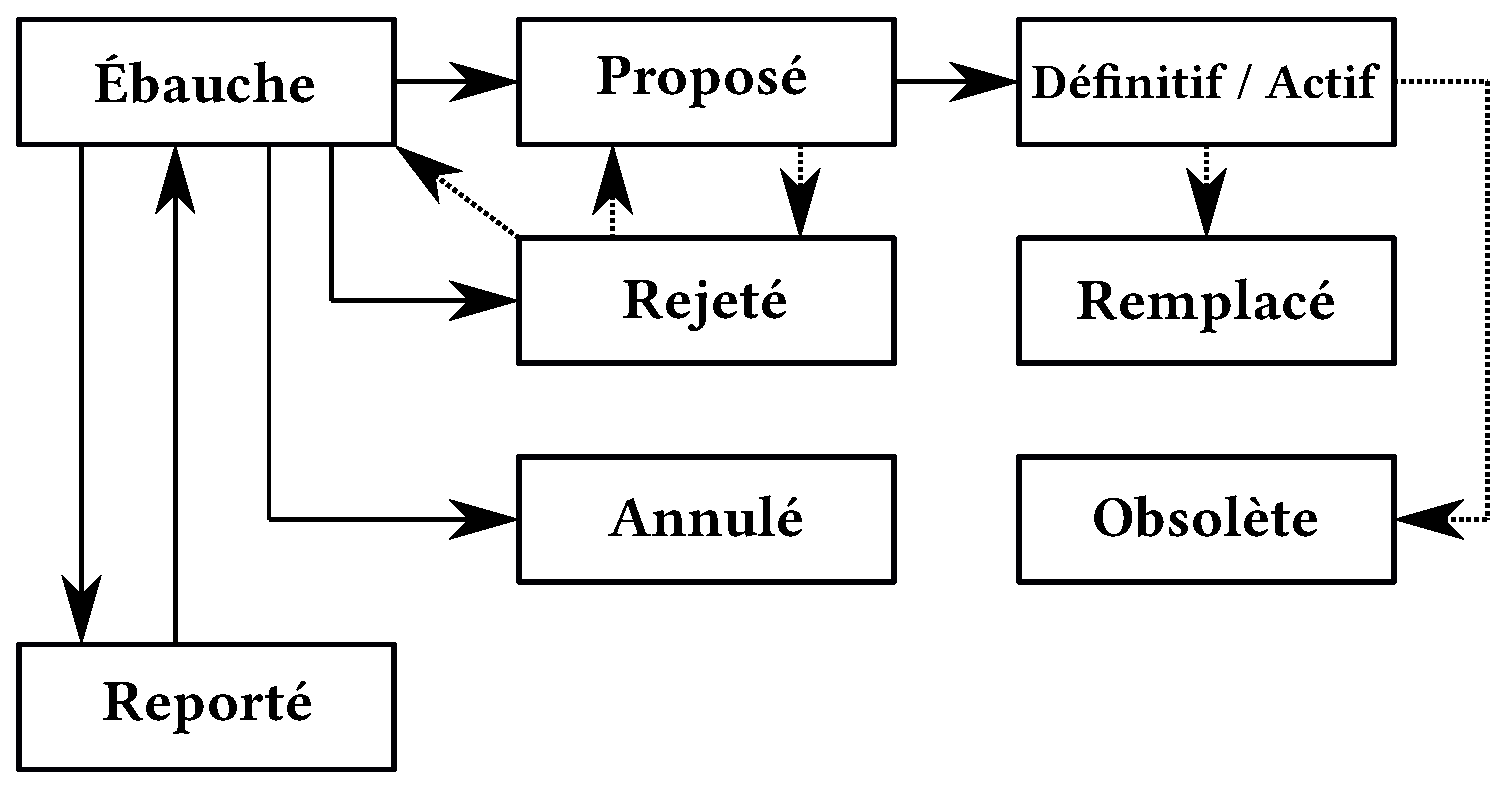
\includegraphics[scale=0.29]{img/bip-process-fr.eps}
  \caption{Schéma de la procédure d'adoption d'un BIP, inspiré du BIP-1.}
\end{figure}

% Utilisation des BIP pour les autres protocoles
Notez que ces documents sont utilisés pour BTC mais également pour d'autres protocoles. Par exemple, les BIP décrivant le fonctionnement des portefeuilles (BIP-32, BIP-39, BIP-44) sont valides pour la grande majorité des cryptomonnaies. Le SLIP-44 recense les cryptomonnaies compatibles avec le BIP-44\sendnote{\url{https://github.com/satoshilabs/slips/blob/master/slip-0044.md}}.

% Autres systèmes de propositions
Les autres protocole cryptoéconomiques disposent même parfois de leurs propres systèmes de proposition. Ethereum utilise les EIP (\eng{Ethereum Improvement Proposals}), Bitcoin Cash les CHIP\sendnote{\url{https://bch.info/en/chips}} (\eng{Cash Improvement Proposals}), Litecoin les LIP\sendnote{\url{https://github.com/litecoin-project/lips}}, etc.

\section*{La vérification des règles de consensus}
\addcontentsline{toc}{section}{La vérification des règles de consensus}

Bitcoin se base sur un réseau public d'ordinateurs accessible librement sur Internet. Ce réseau suit un modèle pair-à-pair, c'est-à-dire un modèle dans lequel tous les membres du réseau, appelés des nœuds, possèdent les mêmes privilèges. Ce sont ces nœuds qui s'assurent que les règles de consensus sont respectées. Si un bloc est invalide (en contenant une transaction invalide par exemple), alors il est rejeté par les nœuds appliquant les règles.

Dans Bitcoin, le rôle des nœuds est d'entretenir une copie du registre des transactions (la fameuse chaîne de blocs) et, ce faisant, de s'assurer de la validité des transactions et des blocs. Pour cela, ils communiquent avec les autres nœuds du réseau et relaient les nouvelles transactions et les nouveaux blocs, qui émanent respectivement des utilisateurs et des mineurs.

% Vérification complète
La vérification des règles de consensus peut être complète. Dans ce cas, on utilise parfois le pléonasme «~nœuds complets~» ou «~\eng{full node}~» pour insister sur le fait qu'ils vérifient l'intégralité de la chaîne. Ils téléchargent l'intégralité de la chaîne de blocs, vérifient les règles de consensus et relaient les blocs et les transactions. C'est une charge~: \textcolor{darkgray}{en avril 2023, la chaîne de Bitcoin pesait environ 480~Go de données et l'ensemble des UTXO plus de 4 Go, la zone mémoire des transactions est limitée à 100~Mo. La taille moyenne des blocs minés toutes les 10 minutes était de 1,3~Mo avant janvier 2023, et gravite aujourd'hui autour de 2~Mo.}

% Nœuds réduits
Les nœuds réduits (\eng{pruned nodes}), qui conservent l'état du réseau mais pas l'entièreté de la chaîne, sont des nœuds à part entière puisqu'ils ont vérifié la conformité des règles sur l'intégralité de la chaîne. Ils ne sont juste pas en mesure d'accéder à l'historique de la chaîne précédant une certaine date.

% Vérification partielle
La vérification peut aussi être partielle, auquel cas on peut parler de client léger (parler de nœud est abusif). Cela est utile pour les personnes qui n'ont pas l'intérêt de faire tourner un nœud complet. C'est par exemple le cas dans les logiciels de hachage (mettant en œuvre Stratum) et dans les portefeuilles légers. Ils utilisent en particulier une méthode conceptualisée dans le livre blanc de Bitcoin en 2008~: la vérification de paiement simplifiée\sendnote{Satoshi Nakamoto décrivait la vérification de paiement simplifiée comme suit~:

\begin{quote}
\footnotesize «~Il est possible de vérifier les paiements sans faire fonctionner un nœud complet du réseau. Un utilisateur a seulement besoin de conserver une copie des entêtes des blocs de la plus longue chaîne de preuves de travail, qu'il peut obtenir en interrogeant les nœuds du réseau jusqu'à ce qu'il soit convaincu qu'il possède la plus longue chaîne, et obtenir la branche de Merkle liant la transaction au bloc dans lequel elle est horodatée. Il ne peut pas vérifier la transaction par lui-même, mais en la reliant à un endroit de la chaîne, il peut voir qu'un nœud du réseau l'a acceptée, et les blocs ajoutés après le confirment.~»
\end{quote}
(Satoshi Nakamoto, \emph{Bitcoin : un système d'argent liquide électronique pair-à-pair}, 31 octobre 2008)}.

% Vérification de paiement simplifiée
La vérification de paiement simplifiée (nommée en anglais \eng{Simplified Payment Verification} et abrégée en SPV) est une méthode astucieuse, conceptualisée dès les origines, qui permet aux utilisateurs néophytes et occasionnels de pouvoir interagir facilement avec le protocole sans devoir gérer un nœud complet, ni devoir faire aveuglément confiance à un dépositaire. Elle permet de réduire considérablement la charge des portefeuilles légers.  % contribue au succès de Bitcoin

% Description de la vérification
La vérification de paiement simplifiée se base sur la façon dont les blocs de transactions sont chaînés et structurés comme on a pu le voir dans le chapitre~\ref{ch:confirmation}. Premièrement, la chaîne de preuve de travail n'est pas à proprement parler une chaîne de blocs, mais une chaîne d'entêtes. Cela fait que les clients légers n'ont qu'à conserver cette chaîne des entêtes pour déterminer la chaîne possédant le plus de travail accumulé. Puisque chaque entête pèse 80 octets, la taille des données à conserver reste modeste pour des appareils modernes~: elle augmente d'environ 4~Mio par an, \textcolor{darkgray}{ce qui représente un peu plus de 60~Mio en avril 2023}.

Deuxièmement, les transactions sont agencées dans un arbre de Merkle, de sorte que les clients légers peuvent se contenter de demander les informations liées à la branche qui les intéressent pour s'assurer de la confirmation d'une de leurs transactions. Le nombre d'empreintes à obtenir et de hachages à effectuer dépend du logarithme binaire ($\log_{2}$) du nombre de transactions présentes dans le bloc. Pour un bloc de 3000 transactions (moyenne haute sur BTC), la charge correspond à demander 12 empreintes de 32 octets et à calculer 12 hachages pour procéder à la vérification.

% Défauts de fiabilité, de confidentialité et de vérification
Cette vérification simplifiée permet d'alléger la charge des portefeuilles, mais elle présente quelques défauts. D'abord, elle manque de fiabilité~: les nœuds ne peuvent pas mentir en inventant une transaction, mais peuvent omettre de transmettre des informations nécessaires. Ce défaut peut être partiellement contrebalancé en augmentant la diversité des connexions sur le réseau. De plus, la vérification est vulnérable si la chaîne est attaquée par une entité disposant de la puissance de calcul majoritaire\sendnote{Ce cas a été décrit par Satoshi Nakamoto dans le livre blanc :

\begin{quote}
\footnotesize «~De ce fait, la vérification est fiable tant que les nœuds honnêtes contrôlent le réseau, mais est plus vulnérable si le réseau est maîtrisé par un attaquant. Alors que les nœuds du réseau peuvent vérifier les transactions par eux-mêmes, la méthode simplifiée peut être trompée par des transactions forgées par l'attaquant aussi longtemps que celui-ci maîtrise le réseau. Une stratégie pour se protéger serait d'accepter les alertes des nœuds du réseau lorsqu'ils détectent un bloc invalide, invitant le logiciel de l'utilisateur à télécharger le bloc complet et les transactions suspectes pour confirmer l'incohérence. Les entreprises qui reçoivent fréquemment des paiements voudront probablement toujours faire fonctionner leurs propres nœuds afin d'obtenir une sécurité plus indépendante et une vérification plus rapide.~»
\end{quote}
(Satoshi Nakamoto, \eng{Bitcoin: A Peer-to-Peer Electronic Cash System}, 31 octobre 2008.)

Les alertes décrites par Satoshi sont aujourd'hui appelées preuves de fraude mais sont toujours en phase de développement.}.

% Défaut de confidentialité
Ensuite, la vérification simplifiée possède aussi une  de confidentialité, en exigeant que le client léger fasse des requêtes auprès des nœuds du réseau et leur dévoile par conséquent son activité transactionnelle\sendnote{Une façon de remédier partiellement à ce problème est d'accroître le nombre d'informations demandées pour dissimuler les informations essentielles. Une première façon de procéder est de mettre en place des filtres de Bloom décrits dans le BIP-37. Il existe également Neutrino, décrit dans le BIP-157 et le BIP-158, qui fait usage du codage de Golomb-Rice et demande une plus grande bande passante.}.

% Défaut de vérification
Enfin, elle présente un défaut de vérification, en étant par définition partielle. Toutes les règles de consensus ne sont pas vérifiées, ce qui fait que les nœuds complets peuvent convenir d'un changement de règle qui ne sera pas remarqué par le client léger. Par exemple, les clients SPV ne vérifient pas les contraintes appliquées sur la taille des blocs, et le réseau pourrait donc subir une modification de cette limite sans qu'ils s'en rendent compte. C'est ce qui explique la stratégie des promoteurs de SegWit2X en 2017, qui prévoyaient de doubler la taille limite des blocs sans protection contre la rediffusion afin que les portefeuilles à vérification de paiement simplifiée suivent simplement la chaîne la plus longue\sendnote{Voir par exemple le courriel de Mike Belshe du 8 octobre 2017 où il déclare~: «~Aujourd'hui, nous sommes en bonne voie pour déployer segwit2x avec une grande majorité de mineurs qui le signalent encore. En plus de cela, 99,94~\% des nœuds et des clients SPV suivront automatiquement la chaîne la plus longue (segwit2x).~» -- Mike Belshe, \eng{[Bitcoin-segwit2x] Strong 2-Way Replay Protection}, \wtime{08/10/2017 20:16:02 UTC}~: \url{https://lists.linuxfoundation.org/pipermail/bitcoin-segwit2x/2017-October/000323.html}.}. % automatically follow that longest chain (segwit2x)

% Avis de Satoshi
Satoshi pensait\sendnote{Satoshi Nakamoto a conservé cette vision jusqu'à son départ, comme en témoigne son courriel à Mike Hearn du 29 décembre 2010~:

\begin{quote}
\footnotesize «~Un jour, lorsque nous aurons des implémentations fonctionnant uniquement en mode client, la taille de la chaîne de blocs n'aura plus beaucoup d'importance. D'ici là, tant que tous les utilisateurs ont toujours à télécharger la chaîne de blocs entière pour commencer, il est bon de pouvoir la maintenir à une taille raisonnable.~»
\end{quote} % "Eventually when we have client-only implementations, the block chain size won't matter much. Until then, while all users still have to download the entire block chain to start, it's nice if we can keep it down to a reasonable size."
(Satoshi Nakamoto, \eng{Re: More BitCoin questions}, \wtime{29/12/2010 21:42 UTC}~: \url{https://plan99.net/~mike/satoshi-emails/thread3.html})} que le système pourrait perdurer avec une vérification centralisée entre les mains de quelques nœuds vérificateurs (dont les mineurs) et que le reste des utilisateurs feraient usage des clients légers. Dans sa première réponse à James A. Donald en novembre 2008, il indiquait ainsi~:

\begin{quote}
«~Bien avant que le réseau n'atteigne cette taille, les utilisateurs pourront utiliser la vérification de paiement simplifiée (section 8) pour contrôler les doubles dépenses, ce qui ne nécessite que la chaîne des entêtes de bloc, soit environ 12~Ko par jour. Seules les personnes essayant de créer de nouvelles pièces auront besoin de faire fonctionner des nœuds de réseau.\sendnote{Satoshi Nakamoto, \eng{Re: Bitcoin P2P e-cash paper}, \wtime{03/11/2008, 01:37:43 UTC}~: \url{https://www.metzdowd.com/pipermail/cryptography/2008-November/014815.html}.}~»
\end{quote} % Long before the network gets anywhere near as large as that, it would be safe for users to use Simplified Payment Verification (section 8) to check for double spending, which only requires having the chain of block headers, or about 12KB per day.  Only people trying to create new coins would need to run network nodes.

En cela, il se trompait. La vérification des règles de consensus a besoin d'être intégrale pour que celles-ci soient appliquées.

% Utilité systémique de cette vérification
C'est donc au niveau du nœud complet que se joue cette vérification, Cette réalité est parfois retranscrite par l'adage «~pas ton nœud, pas tes règles\sendnote{L'adage «~\eng{not your node, not your rules}~» a été naturellement calqué sur l'adage «~\eng{not your keys, not your coins}~» (voir par exemple ce tweet de Udi Wertheimer~: \url{https://twitter.com/udiWertheimer/status/936215582487261184}). Il a été popularisé par le panel du même nom lors de la conférence Understanding Bitcoin, le 5 avril 2019~: \url{https://www.youtube.com/watch?v=jwaKVIEm-rI}. Le projet RaspiBlitz en a fait son slogan en 2020~: \url{https://github.com/rootzoll/raspiblitz/blob/bbeb5b21a982eeeb93306537e0aca2474bd23e03/README.md}.}~». Ne faites pas confiance, vérifiez~! Tout comme une langue résulte des choix que font ses locuteurs (n'en déplaise à l'Académie Française), un protocole informatique résulte des règles appliquées par les nœuds complets. Cette vérification joue donc un rôle crucial dans la détermination du protocole.

\section*{Les hard forks}
\addcontentsline{toc}{section}{Les hard forks}

Avant de voir comment est spécifiquement déterminé le protocole, intéressons-nous aux modifications des règles de consensus et comment elles se manifestent. Les modifications des règles de consensus peuvent être rangées dans deux catégories~: les \eng{hard forks}, mises à niveau brutes et incompatibles, et les soft forks, qui présentent une certaine rétrocompatibilité.

% Polysémie du mot fork
Le mot \eng{fork} est un terme anglais signifiant «~embranchement~», «~bifurcation~» ou «~fourche~». Dans Bitcoin, il existe une polysémie à son sujet (le terme possède quatre significations différentes), ce qui peut prêter à confusion.

% Fork logiciel
Comme on l'a dit, le terme de fork est d'abord utilisé dans le développement logiciel, notamment dans le cadre du logiciel libre qui autorise et encourage ce type de pratique. Il désigne la création un programme dérivé du code source d'un programme existant et aussi, par abus de langage, le programme dérivé en lui-même. En ce sens, l'implémentation de référence peut subir un embranchement, créant un logiciel alternatif. Ce logiciel peut respecter les règles de consensus (comme par exemple Bitcoin Knots), mais il peut aussi les faire dévier, en créant un nouveau protocole qui partage l'historique de la chaîne (Bitcoin ABC, devenu Bitcoin Cash Node) ou non (Litecoin).

% Embranchement commun de la chaîne
Le fork peut ensuite désigner l'embranchement commun de la chaîne de blocs, par analogie avec le développement logiciel. La chaîne de blocs n'est en effet pas une structure linéaire, mais une «~structure en forme d'arbre\sendnote{Satoshi Nakamoto, code source de la version 0.1 du logiciel Bitcoin~: \url{https://github.com/trottier/original-bitcoin/blob/4184ab26345d19e87045ce7d9291e60e7d36e096/src/main.h\#L1001-L1008}.}~» qui peut posséder de multiples branches de blocs, pareillement compatibles avec les règles de consensus acceptées par le réseau, la sélection de la branche correcte se faisant par la plus longue (possédant le plus de travail accumulé). Ce type d'embranchement se produit régulièrement dans Bitcoin de manière tout à fait normale et bénigne, lorsque deux mineurs trouvent simultanément un bloc différent de leur côté, et est résolu lorsqu'un nouveau bloc est trouvé.

% Scission
Le fork peut aussi se rapporter à une scission de la chaîne de blocs causée par une incompatibilité des règles de consensus. On parle alors de hard fork, c'est-à-dire littéralement d'«~embranchement dur~». Cette scission est généralement permanente dans le sens où les deux branches ne peuvent pas se réconcilier par le mécanisme de consensus de Nakamoto, sauf dans un cas très précis~: si les règles de la branche majoritaire forment une restriction des règles de la branche minoritaire. Les deux chaînes résultantes sont, à terme, vouées à exister sur des réseaux séparés.

% Hard fork / soft fork
Enfin, le terme de fork peut, par métonymie, désigner une modification des règles de consensus, qui est toujours susceptible de provoquer une scission de chaîne et une séparation du réseau. Une restriction des règles de consensus est appelée un soft fork, littéralement «~embranchement doux~», en vertu de sa capacité à ne résulter en une branche unique. Toute autre modification des règles de consensus, qu'il s'agisse d'une extension ou d'une modification strictement incompatible, est appelée un hard fork, en référence à sa propension à créer une scission de chaîne. C'est de ces deux modifications dont nous voulons parler ici.\sendnote{Notez que les concepts sont liés. Ainsi, un fork logiciel (copie et modification) peut implémenter un fork des règles de consensus (hard fork ou soft fork) qui finira par créer un fork de chaîne (scission).}

%
Le hard fork est le concept le plus ancien chronologiquement par rapport au soft fork. Il était auparavant qualifié de «~changement incompatible\sendnote{Voir par exemple David François, \eng{Re: Small protocol changes for flexibility}, \wtime{07/12/2010 15:08:02 UTC}~: \url{https://bitcointalk.org/index.php?topic=894.msg27757\#msg27757}.}~». Le hard fork est une modification non restrictive des règles de consensus. Il provoque un conflit sur le réseau entre les nœuds qui appliquent les anciennes règles et les nœuds qui appliquent les nouvelles.

% Hard fork extensif
Un hard fork peut être extensif, c'est-à-dire élargir les règles de consensus sur les blocs et les transactions. Les anciens peuvent ainsi produire des blocs valides sur la nouvelle chaîne, mais pas l'inverse. L'exemple typique de ce genre de hard fork est l'augmentation de la taille limite des blocs, qui consiste à accepter des blocs ayant une taille ou un poids plus grand. Par exemple, un passage de 1~Mo à 2~Mo ou de 4~MWU à 8~MWU.

\textcolor{brown}{schéma hard fork extensif d'augmentation de la taille limite de blocs, branche majoritaire}

Dans le cas où le hard fork extensif n'est pas soutenu par une majorité de la puissance de calcul du réseau, celui-ci risque de ne pas avoir lieu. En effet, les blocs de la branche imposant une taille plus petite sont entièrement compatibles avec les nouvelles règles, de sorte que, si elle est plus longue, c'est elle qui sera sélectionnée comme la branche correcte. C'est pour éviter cette situation problématique que les hard forks sont généralement bilatéraux.

% Hard fork bilatéral
Mais il peut aussi être bilatéral en créant une incompatibilité totale entre les nouvelles règles et les anciennes. Il peut s'agir d'une règle ajoutée comme l'exigence que le premier bloc de l'embranchement inclue un changement incompatible. Dans notre cas de l'augmentation de la chaîne de blocs, il s'agirait d'imposer au premier bloc d'être strictement plus gros que la taille limite précédente. Cette règle supplémentaire est appelée protection contre la destruction par recoordination (\eng{wipeout protection}).

\textcolor{brown}{schéma hard fork bilatéral d'augmentation de la taille limite de blocs, branche minoritaire}

Un autre exemple est le changement de l'algorithme de signature des transactions, qui rend l'intégralité des transactions signées et des blocs non vides strictement incompatibles. Ce changement a pour effet de permettre en plus une protection contre la rediffusion des transactions (\eng{replay protection}), dans le cas où deux chaînes concurrentes persisteraient.

% Deux hard forks, deux intentions
Deux situations peuvent découler d'un hard fork~: soit la quasi-totalité de l'économie procède au changement, auquel cas une seule chaîne subsiste~; soit l'économie se fragmente, auquel cas les deux chaînes subsistent. La première situation est visée par le hard fork de mise à niveau qui n'a pas vocation à créer deux chaînes distinctes. La seconde est désirée par le hard fork contentieux, résultant d'une division de la communauté au sujet du changement. Le hard fork accidentel, créé par une modification non désirée des règles de consensus implicites, est écarté ici\sendnote{Le 11 mars 2013, le passage de la version 0.7 du logiciel à la version 0.8 implémentait la migration du système de base de données de Berkeley DB à LevelDB. Toutefois, il s'avérait que Berkeley DB faisait intervenir une limite par défaut (\eng{lock limit}) qui n'était pas présente dans LevelDB. Par conséquent, la migration constituait un hard fork accidentel et a provoqué un embranchement à partir du bloc 225~430 qui a duré environ 6 heures. La décision a finalement été prise de revenir à la version 0.7, invalidant la branche de 24 blocs minée du côté de la version 0.8, et de procéder à la migration quelques mois plus tard. -- Voir Vitalik Buterin, \eng{Bitcoin Network Shaken by Blockchain Fork}, 13 mars 2013~: \url{https://bitcoinmagazine.com/technical/bitcoin-network-shaken-by-blockchain-fork-1363144448}~; Gavin Andresen, \eng{BIP-50: March 2013 Chain Fork Post-Mortem}, ~: \url{https://github.com/bitcoin/bips/blob/master/bip-0050.mediawiki}. Une double dépense conséquente a été réalisée~: macbook-air, \eng{A successful DOUBLE SPEND US\$10000 against OKPAY this morning.}, \wtime{12/03/2013, 18:22:02 UTC}~: \url{https://bitcointalk.org/index.php?topic=152348.msg1616747\#msg1616747}.}.

% Hard fork de mise à niveau
Le hard fork de mise à niveau est un hard fork qui nécessite une synchronisation de la quasi-totalité de la communauté. Il résulte généralement en une seule chaîne, de sorte qu'on peut considérer que le protocole a été mis à niveau (alors qu'il s'agit essentiellement d'une utilisation économique qui passe d'un protocole à un autre). Il peut pour cela être extensif, même la bilatéralité est préférée pour des raisons de sécurité.

% Exemples de hard forks de mise à niveau
Le premier hard fork de mise à niveau connu est probablement l'ajout par Satoshi Nakamoto des codes opération \texttt{OP\_NOP} à la version 0.3.6 de Bitcoin en juillet 2010. L'augmentation de la taille des blocs était également pensée comme un hard fork de mise à niveau, notamment par Satoshi Nakamoto lui-même\sendnote{En octobre 2010, à la suite de la proposition de Jeff Garzik d'augmenter la limite directement à 7,168~Mo afin d'«~égaler le taux transactionnel moyen de PayPal~», Satoshi -- bien conscient qu'il s'agissait d'un correctif «~incompatible avec le réseau~» -- écrivait~:
\begin{quote}
\footnotesize «~[La mise à niveau] peut être introduite progressivement, par exemple~:

if (blocknumber > 115000)
  maxblocksize = largerlimit

Elle peut commencer à être intégrée dans les versions bien avant, de sorte qu'au moment où elle atteint le numéro de bloc et entre en vigueur, les anciennes versions qui ne l'ont pas sont déjà obsolètes.

Lorsque nous approchons du numéro de bloc limite, je peux envoyer une alerte aux anciennes versions pour qu'elles sachent qu'elles doivent effectuer une mise à jour.~»
\end{quote}
(Satoshi Nakamoto, \eng{Re: [PATCH] increase block size limit}, \wtime{04/10/2010 19:48:40 UTC}~: \url{https://bitcointalk.org/index.php?topic=1347.msg15366\#msg15366})}, jusqu'au hard fork contentieux de Bitcoin Cash en 2017.

En dehors de BTC, les mises à niveaux par hard fork sont nombreuses, notamment en raison d'une économie moins grande et~/~ou plus centralisée. On peut citer les cas de Bitcoin Cash, de Monero, d'Ethereum Classic et d'Ethereum, où des mises à niveau de ce type sont réalisées régulièrement.

% Hard fork contentieux
Le hard fork contentieux est un hard fork visant à créer une nouvelle chaîne délibérément. Il est issu d'une dissension dans la communauté, si forte qu'elle pousse à la sécession. Il est généralement bilatéral.

% Exemples de hard forks contentieux
Le premier exemple de hard fork contentieux majeur est celui qui a eu lieu sur Ethereum en juillet 2016, dans le contexte du piratage de TheDAO. Ce hard fork consistait à reprendre les fonds du pirate par un «~changement d'état irrégulier~». Celui-ci était rendu bilatéral par la règle imposant aux 10 premiers blocs d'inclure la chaîne de caractères \texttt{dao-hard-fork}. Puisque la majorité économique se trouvait du côté de l'annulation, la chaîne altérée a gardé le nom d'Ethereum et le sigle boursier ETH, tandis que l'autre chaîne a pris le nom d'Ethereum Classic et le sigle boursier ETC.\sendnote{Simon Polrot, \emph{The DAO~: post mortem}, 24 janvier 2017~: \url{https://www.ethereum-france.com/the-dao-post-mortem/}~; Casey Detrio, \eng{EIP-779: Hardfork Meta: DAO Fork}, 26 novembre 2017~: \url{https://eips.ethereum.org/EIPS/eip-779}.}

Le second exemple de hard fork contentieux est celui qui a mené à la création de Bitcoin Cash en août 2017 suite au débat sur la scalabilité et à la guerre des blocs. Ce hard fork n'intégrait pas SegWit, augmentait la taille limite des blocs à 8~Mo et améliorait l'algorithme de signature. Il était rendu bilatéral par une règle qui imposait au bloc suivant l'activation d'avoir une taille au bloc suivant d'avoir une taille strictement supérieure à 1~Mo. Il offrait aussi \emph{de facto} une protection contre la rediffusion des transactions. Ce changement ayant dû se faire sans l'accord de la majorité économique, la chaîne qui ne modifiait pas les règles a pu conserver le nom de Bitcoin et le sigle boursier BTC, tandis que la nouvelle chaîne a dû adopter un nouveau nom, Bitcoin Cash, et un nouveau sigle BCH.\sendnote{Ludovic Lars, \emph{Bitcoin Cash~: la branche minoritaire issue du débat sur la scalabilité}, 30 janvier 2022~: \url{https://journalducoin.com/analyses/bitcoin-cash-branche-minoritaire-debat-scalabilite/}~; \eng{BCH-UAHF: Bitcoin Cash User-Activated Hard Fork}, 24 juillet 2017~: \url{https://reference.cash/protocol/forks/bch-uahf}.}

\textcolor{brown}{schéma scission Bitcoin / Bitcoin Cash}

% Ajustement de la difficulté
Notez qu'un tel hard fork peut devoir avoir à modifier l'algorithme d'ajustement de difficulté. En effet, si la puissance de calcul est trop faible pour le soutenir, il est possible que l'ajustement n'arrive pas à terme. C'est pour cette raison que Bitcoin Cash a dû implémenter un \eng{Emergency Difficulty Adjustment} (EDA) qui a permis de procéder à l'adaptation sur une période plus courte. Ethereum Classic n'a cependant pas dû le faire, car l'ajustement sur Ethereum avait déjà lieu à tous les blocs.

\section*{Les soft forks}
\addcontentsline{toc}{section}{Les soft forks}

% Définition
Le soft fork est une restriction des règles de consensus. Il consiste par essence à rendre l'ensemble des blocs et des transactions valides plus petit, en ajoutant une règle ou en modifiant une règle existante de façon plus restrictive. L'exemple typique de ce genre de fork est la diminution de la taille limite des blocs. L'ajout de la limite explicite des 1~Mo en octobre 2010 était ainsi un soft fork.

% Application par la puissance de calcul
Le soft fork peut être appliqué en conservant une seule et même chaîne. S'il est imposé par la majorité de la puissance de calcul du réseau, il n'y a aucun risque de scission. En effet, l'ensemble des blocs créés par les mineurs appliquant les nouvelles règles est entièrement compatible avec les anciennes règles, de sorte que la branche appliquant les nouvelles règles sera considérée comme la branche correcte par tous les nœuds si elle est majoritaire.

\textcolor{brown}{schéma soft fork de diminution de la taille limite de blocs, branche majoritaire}

% Origine
Le concept de soft fork est postérieur à celui de hard fork. Il a été formellement découvert par Gavin Andresen en octobre 2011 qui, suite à son étude de la proposition d'ajout du code opération \texttt{OP\_EVAL} par Nicolas van Saberhagen\sendnote{Nicolas van Saberhagen, \eng{OP\_EVAL proposal}, \wtime{02/10/2011 00:49:19 UTC}~: \url{https://bitcointalk.org/index.php?topic=46538.msg553689\#msg553689}.}, s'est aperçu que la mise à niveau pouvait se faire grâce aux code opération \texttt{OP\_NOP1} sans nécessairement provoquer de scission\sendnote{«~Je lis probablement mal le code, mais je pense que OP\_EVAL ne provoquerait pas de scission de blockchain~!~» s'est exprimé Gavin Andresen sur IRC. -- \#bitcoin-dev IRC logs, 2 octobre 2010~: \url{https://web.archive.org/web/20131201200245/http://bitcoinstats.com/irc/bitcoin-dev/logs/2011/10/02}.}.

% Codes opération
Les codes opération \texttt{OP\_NOP} sont des instructions du langage de script de Bitcoin qui ont été ajoutés dans le code par Satoshi en juillet 2010 avec pour seul commentaire «~expansion\sendnote{\url{https://sourceforge.net/p/bitcoin/code/119/}}~». Le changement a été rendu effectif avec la version 0.3.6 du logiciel qui corrigeait également le 1 RETURN bug, publiée le 29 juillet\sendnote{Satoshi Nakamoto, \eng{*** ALERT *** Upgrade to 0.3.6}, \wtime{29/07/2010 19:13:06 UTC}~: \url{https://bitcointalk.org/index.php?topic=626.msg6451\#msg6451}.}. Leur rôle est initialement muet~: s'ils sont présents dans un script, ils ne font rien mais ils n'invalident pas la transaction non plus. Cela entraîne qu'on peut modifier le comportement de ces codes opération sans rendre les scripts incompatibles avec les anciennes règles de consensus. Cette caractéristique indique que que Satoshi avait, sinon compris, au moins deviné le mécanisme du soft fork.

% Échange sur IRC
% 16:40	gavinandresen	I'm probably reading the code wrong, but I think OP_EVAL wouldn't cause a blockchain split!
% 18:59	gmaxwell	wow. Gavin's point that EVAL can be done without a split blew my mind.
% 21:23	gmaxwell	You can also make the new code keep the old behavior for blocks before a certian height.
% 21:24	gmaxwell	So you can set the actual switch point at some point in the future.
% 21:25	gmaxwell	(so that you have time to actually achieve >>50% hashpower behind the change)
% 21:27	gmaxwell	e.g. make and backport a patch which will agressively not forwardward txn with the reserved NOP until block X, and after X start applying the new validation rules but only to future blocks. Then so long has >>50% hashpower is running this patch by block X there is no lasting fork created.

% Caractère postcompatible
Le soft fork possède un caractère «~rétrocompatible~» -- ou postcompatible à proprement parler, la compatibilité étant ascendante et non descendante -- dans le sens où les anciennes versions du logiciel peuvent continuer d'interagir avec le système. En effet, les nœuds non miniers suivant les anciennes règles continuent de voir les blocs produits comme valides. Cette caractéristique est un avantage majeur par rapport au hard fork.

% La rétrocompatibilité, ou compatibilité descendante, est la compatibilité d'un produit vis-à-vis de ses anciennes ou précédentes versions ; la compatibilité ascendante ou postcompatibilité est la compatibilité d'un produit vis-à-vis des versions plus récentes, voire encore en phase de conception.

% Non-optionnalité
Mais cette compatibilité ascendante ne veut pas dire qu'un soft fork est «~doux~». Il possède un côté pernicieux dans le sens où il rend la modification difficile à appréhender. D'abord, il n'est pas optionnel. S'il est appliqué par la majorité de la puissance de calcul, un soft fork s'apparente en effet à une attaque de censure pour les utilisateurs appliquant les anciennes règles. Le soft fork possède donc un caractère coercitif que le hard fork n'a pas.

% Irréversibilité
Puis, le soft fork est difficilement réversible. Les fonctionnalités ajoutées ne peuvent pas être désactivées simplement~: une fois adopté, il n'y a pas de retour en arrière facile. Les développeurs de Bitcoin SV ont ainsi désactivé P2SH en février 2020 exposant les utilisateurs les moins attentifs à des vols\sendnote{Jon Southurst, \eng{Final Genesis specs released—bye P2SH}, 10 janvier 2020~: \url{https://coingeek.com/final-genesis-specs-released-bye-p2sh/}.}.

% Non-limitation
Ensuite, le soft fork n'est pas limité quant à ce qu'il peut faire. Il peut augmenter la limite effective de taille des blocs (via un bloc auxiliaire aussi appelé bloc d'extension\sendnote{\url{https://bitcointalk.org/index.php?topic=283746.msg3036293\#msg3036293}~; \url{https://lists.linuxfoundation.org/pipermail/bitcoin-dev/2015-May/008356.html}} ou soft fork généralisé\sendnote{ZoomT, \eng{Increasing the blocksize as a (generalized) softfork.}, \wtime{20/12/2015 11:12:48 UTC}~: \url{https://bitcointalk.org/index.php?topic=1296628.msg13305141\#msg13305141}.}). Ce bloc d'extension peut également inclure des fonctionnalités supplémentaires (comme MimbleWimble dans Litecoin). Il peut même modifier la politique monétaire du protocole en redéfinissant l'unité de base\sendnote{La façon dont un soft fork peut introduire de l'inflation dans Bitcoin a été exposée par le développeur Peter Todd en 2016. -- Peter Todd, \eng{Forced Soft Forks}, 18 janvier 2016~: \url{https://petertodd.org/2016/forced-soft-forks}.}.

% Complexité
Enfin, le soft fork, s'il est profond, crée une complexité supplémentaire, liée aux contraintes de son application. En effet, il ajoute de nouvelles exceptions aux règles de consensus, ce qui génère de la dette technique\sendnote{Ward Cunningham, «~The WyCash Portfolio Management System~», \eng{Addendum to the Proceedings of OOPSLA 1992}, octobre 1992~: \url{https://dl.acm.org/doi/pdf/10.1145/157710.157715}.} pour les développeurs.

% (L'abominable) SegWit
L'archétype du soft fork profond et complexe a été la mise à niveau SegWit, ou \eng{Segregated Witness}, qui consistait à déplacer les données de signature des transactions (appelées témoin ou \eng{witness}) vers une structure de données séparée (\eng{segregated}) afin de supprimer la malléabilité des transactions. Cette mise à niveau, qui a eu lieu en le 24 août 2017, devait être initialement un hard fork, avant que le développeur luke-jr ne décrive en 2015 comment en faire un soft fork\sendnote{Aaron van Wirdum, \eng{The Long Road to SegWit: How Bitcoin's Biggest Protocol Upgrade Became Reality}, 23 août 2017~: \url{https://bitcoinmagazine.com/technical/the-long-road-to-segwit-how-bitcoins-biggest-protocol-upgrade-became-reality}.}. La rétrocompatibilité était assurée par la liaison du témoin au bloc via un arbre de Merkle dont la racine était placée dans la transaction de récompense et par l'utilisation de sorties transactionnelles dépensables par n'importe qui (\eng{anyone-can-spend}). Outre la correction du problème de malléabilité, elle a instauré un système de versionnage (qui a permis l'intégration de Schnorr-Taproot par la suite) et a modérément augmenté la capacité transactionnelle du réseau, de sorte que la taille effective des blocs pouvait dépasser 1~Mo, jusqu'à 4~Mo en théorie. Elle a également ajouté quatre nouveaux types d'adresse au protocole.

% Méthodes d'activation
De plus, le soft fork requiert la majorité de la puissance de calcul du réseau pour préserver son intérêt. S'il n'est pas suivi à moyen terme par 51~\% de la puissance de calcul, alors son application provoque une scission. C'est ce qui explique pourquoi l'activation par les mineurs est généralement préférée à l'activation par les utilisateurs, même si le pouvoir de décision revient à ces derniers comme on le verra.

% Soft fork activé par les utilisateurs
D'une part, le soft fork activé par les utilisateurs (en anglais \eng{user activated soft fork} ou UASF) consiste à implémenter le soft fork dans le code source du logiciel de sorte à ce qu'il rentre en application à une hauteur de bloc ou à un horodatage donné. Cette méthode s'appuie sur la confiance que l'économie appliquant la mise à niveau sera largement majoritaire et que l'activité minière suivra à moyen terme en raison d'une récompense de bloc plus élevée.

% Soft fork activé par les mineurs
D'autre part, le soft fork activé par les mineurs (en anglais \eng{miner activated soft fork} ou MASF) consiste à faire dépendre l'activation du signalement des mineurs au sein des blocs validés. Il est activé lorsqu'un certain seuil de signalement (95~\% par exemple) est dépassé. Cette méthode, dont la procédure a été notamment décrite dans le BIP-9, permet de s'assurer autant que possible que les mineurs appliquent la mise à niveau et qu'il ne subsiste qu'une seule chaîne.

% UAHF / MAHF
La même distinction existe dans l'activation des hard forks, mais celle-ci peu de pertinence, la puissance de calcul ne pouvant pas empêcher la scission. Ainsi, le hard fork activé par les mineurs (MAHF), longtemps été soutenu par les partisans de l'augmentation de la taille limite des blocs, n'a pas d'intérêt particulier.

% Deux types de soft forks
Comme les hard forks, les soft forks peuvent être rangés en deux catégories plus ou moins distinctes~: le soft fork de mise à niveau et le soft fork contentieux.

% Soft fork de mise à niveau
Le soft fork est idéal pour mettre à niveau le protocole. Cela permet aux nœuds de ne pas se mettre à niveau tout de suite. Même s'il demande une certaine synchronisation, celle-ci n'est pas aussi contraignante que pour les hard forks.

% Exemples de soft forks de mise à niveau dans BTC
Dans BTC, le soft fork est ainsi privilégié par les développeurs depuis sa découverte. De nombreuses mises à niveau en étaient, comme \eng{Pay to Script Hash} (BIP-16), ou l'obligation de spécifier la hauteur du bloc dans la transaction de récompense (BIP-34), ou encore l'ajout d'un standard d'encodage des signatures (BIP-66). Les ajouts des codes opération \texttt{OP\_CHECKLOCKTIMEVERIFY} et \texttt{OP\_CHECKSEQUENCEVERIFY} permettant l'usage de verrous temporels dans le langage de scipt par l'utilisation respective des codes \texttt{OP\_NOP2} et \texttt{OP\_NOP3} ont également été des soft forks. Enfin, plus récemment, l'adoption de Schnorr-Taproot (ou Taproot pour faire court) a été une mise à niveau par soft fork.

% Exemples de soft forks de mise à niveau dans LTC
Litecoin fait aussi usage de ce type de transition. Le protocole a notamment intégré SegWit en mai 2017, ainsi que Schnorr-Taproot et MimbleWimble (MWEB) en mai 2022.

% Soft fork contentieux
Le soft fork contentieux a pour objectif de contraindre la minorité de la communauté à suivre la majorité. S'il réussit, il n'y a qu'une seule chaîne, les opposants ayant le choix d'accepter les règles ou de procéder eux-mêmes à un hard fork. S'il échoue, il résulte en deux chaîne concurrentes.

% SegWit
SegWit est l'exemple typique d'un soft fork contentieux réussi. Il n'était pas approuvé par l'ensemble des acteurs importants (les partisans des gros blocs d'une part, les puristes du protocole comme Mircea Popescu d'autre part, s'y opposaient), mais il a recueilli un soutien majoritaire de sorte qu'il a pu perdurer et que les mécontents \eng{big blockers} ont dû migrer vers Bitcoin Cash.

% "Coinbase rule"
Un exemple de soft fork contentieux ayant échoué est la tentative de l'équipe de Bitcoin ABC d'imposer une redirection de 8~\% de la subvention de minage de Bitcoin Cash vers elle-même le 15 novembre 2020\sendnote{Amaury Séchet, \eng{Bitcoin ABC's plan for the November 2020 upgrade}, 6 août 2020~: \url{https://amaurysechet.medium.com/bitcoin-abcs-plan-for-the-november-2020-upgrade-65fb84c4348f}.}. Cette tentative, qui était un soft fork en raison du caractère restrictif, a provoqué la scission entre une branche majoritaire sans redirection (BCH) et une branche minoritaire avec, qui a été par la suite renommée en «~eCash~» (XEC).

% Supériorité du soft fork
Ainsi, le soft fork, qu'il soit approuvé à l'unanimité ou bien seulement par une majorité, est une méthode supérieure au hard fork. Bien qu'il soit parfois plus complexe, il permet de ne pas requérir une synchronisation de l'économie entière, cette dernière pouvant s'y adapter progressivement, ce qui est un bienfait non négligeable dans le cas d'un système ouvert et divers comme Bitcoin. Le signalement supermajoritaire des mineurs permet de minimiser le risque de scission et de conserver l'effet de réseau au maximum.

% % Meilleure méthode de mise à niveau
% Les soft forks ont ainsi des caractéristiques précises qui font qu'ils possèdent des avantages, mais aussi des inconvénients, par rapport aux hard forks. Si la mise à niveau est profonde, le hard fork a l'avantage d'être simple, tandis que le soft fork peut présenter une certaine complexité. Le hard fork requiert que l'ensemble du réseau se synchronise pour appliquer la mise à niveau, tandis que le soft fork ne demande qu'une synchronisation de la puissance de calcul majoritaire et une adaptation progressive de l'économie. De ce fait, la probabilité d'une scission est plus élevée dans le cas d'un hard fork que dans celui d'un soft fork qui aurait fait l'objet d'un signalement supermajoritaire des mineurs, ce qui permet la conservation de l'effet de réseau.

% Sacrifice du consentement
Mais cet avantage majeur se fait au prix d'un sacrifice~: celui de la clarté du consentement. Dans le cas du hard fork, le consentement est clair~: les personnes qui souhaitent la modification se retrouvent sur la chaîne qu'elles ont choisie. Dans le cas, du soft fork, le consentement est plus ambigu~: le fait d'opérer sur la chaîne n'indique pas nécessairement une acceptation active du changement, mais une résignation passive et un refus de réaliser un hard fork minoritaire. Comme l'écrivait brillamment Vitalik Buterin en mars 2017~:

\begin{quote}
«~Les soft forks favorisent clairement la coercition par rapport à la sécession d'un point de vue systémique, alors que les hard forks ont le penchant inverse.\sendnote{Vitalik Buterin, \eng{Hard Forks, Soft Forks, Defaults and Coercion}, 14 mars 2017~: \url{https://vitalik.ca/general/2017/03/14/forks_and_markets.html}.}~»
\end{quote} % Soft forks clearly institutionally favor coercion over secession, whereas hard forks have the opposite bias.

Ainsi, même s'ils sont supérieurs dans la plupart des cas, les soft forks ne doivent pas nécessairement être privilégiés dans toutes les situations.

\section*{Le pouvoir sur le protocole} % Le rôle central des commerçants
\addcontentsline{toc}{section}{Le pouvoir sur le protocole}

La détermination du protocole est un aspect majeur de Bitcoin. En effet, l'absence d'autorité centrale pose la question de la prise de décision~: puisqu'il n'y a personne pour ordonner quoi que ce soit, comment le protocole peut-il être choisi et modifié~? Il est donc nécessaire de repenser notre conception de la chose pour pouvoir la comprendre.

% Détermination économique
Tel que nous l'avons laissé entendre, la détermination du protocole est réalisée par l'économie. Puisque Bitcoin est un système économique, il est naturel que les règles qui le composent résultent du marché, et non d'un décret fixe passé ou d'une autorité centrale actuelle.

L'idée que l'économie permet de déterminer le protocole n'est pas nouvelle, et remonte au moins à la déclaration de Meni Rosenfeld qui écrivait dans une réponse sur Stack Overflow en juin 2012 qu'un changement du protocole nécessitait «~une majorité économique, c'est-à-dire l'adoption par les utilisateurs et les entreprises qui donnent de la valeur à la monnaie\sendnote{\url{https://bitcoin.stackexchange.com/questions/3945/how-could-the-bitcoin-protocol-be-changed-has-this-ever-occurred\#comment4983_3948}}~». Gavin Andresen lui-même avait mis en avant cette idée en mai 2015, alors que la question d'augmenter la taille limite des blocs se posait~: % "A change requires an economic majority - adoption by the users and businesses who give the currency value."

\begin{quote}
«~Si nous ne parvenons pas à un consensus ici, l'autorité ultime pour déterminer le consensus est le code utilisé par la majorité des commerçants, des plateformes d'échange et des mineurs.\sendnote{Gavin Andresen, \eng{[Bitcoin-development] Proposed alternatives to the 20MB step function}, \wtime{29/05/2015 12:39:30 UTC}, \url{https://lists.linuxfoundation.org/pipermail/bitcoin-dev/2015-May/008340.html}.}~»
\end{quote} % "Because if we can't come to consensus here, the ultimate authority for determining consensus is what code the majority of merchants and exchanges and miners are running."

Mais la clarté de cette conception n'est arrivée qu'après les évènements de la guerre des blocs, durant laquelle les mécanismes sous-jacents ont pu s'exprimer. Ce n'étaient pas les développeurs qui décidaient des règles, ce n'étaient pas les mineurs non plus, mais bien plutôt les utilisateurs, et plus précisément les \emph{commerçants}. Eric Voskuil écrivait ainsi en novembre 2018~:

\begin{quote}
«~Bitcoin ne repose pas sur un dépositaire, mais dans l'intérêt d'établir un principe général, on peut considérer l'ensemble de tous les commerçants comme le dépositaire collectif de Bitcoin.\sendnote{Eric Voskuil, \emph{Cryptoéconomie}, «~Principe de risque de garde~» (p. 34).}~»
\end{quote}

% Le pouvoir des commerçants
Les commerçants sont, au sens large, les personnes qui fournissent des biens, des services ou d'autres monnaies contre du bitcoin, à des prix acceptables sur le marché. Cette prestation se manifeste par les échanges effectifs avec des clients et se mesure au travers des recettes perçues. En cela, les commerçants contribuent à l'utilité du bitcoin, qui se mesure à la quantité de biens et de services qu'il permet d'acquérir, et par conséquent à l'importance économique de la chaîne\sendnote{Cette réalité avait été perçue en janvier 2010 par NewLibertyStandard, le premier commerçant de Bitcoin~: «~Toutes les personnes qui achètent ou vendent des biens en utilisant des bitcoins, y compris les changeurs, font progresser l'économie de Bitcoin~!~» -- NewLibertyStandard, \eng{Re: New Exchange Service: "BTC 2 PSC"}, \wtime{19/01/2010 08:06:15 UTC}~: \url{https://bitcointalk.org/index.php?topic=15.msg111\#msg111}.}. Par l'utilisation d'un nœud permettant de vérifier les règles de consensus, ils participent ainsi à la détermination du protocole en proportion de leur activité économique potentielle.

% Modifier le protocole
Parler d'un protocole unique qui changerait est une approximation~: en tant qu'ensemble de règles, les protocoles sont tous fixes, mais leur utilisation (et leur utilité) varie. Modifier le protocole consiste donc à constituer un nouveau protocole dont la chaîne résultante sera économiquement plus importante que toute autre branche concurrente, y compris celle liée au protocole originel\sendnote{Jeff Garzik écrivait très justement en octobre 2010 que «~l'effort visant à augmenter la limite du taux de transaction [était] le même que celui visant à modifier la nature fondamentale des bitcoins~: convaincre la grande majorité de se mettre à niveau~». -- Jeff Garzik, \eng{Re: [PATCH] increase block size limit}, \wtime{04/10/2010 18:33:55 UTC}~: \url{https://bitcointalk.org/index.php?topic=1347.msg15342\#msg15342}.}. Par exemple, SegWit a été un soft fork contentieux, mais le protocole résultant a été beaucoup plus valorisé que les protocoles concurrents (BTC pré-SegWit et Bitcoin Cash), de sorte qu'on peut dire que le protocole BTC a été mis à niveau par cette modification. % The effort to raise the transaction rate limit is the same as the effort to change the fundamental nature of bitcoins:  convince the vast majority to upgrade.

% Multiplicité des Bitcoins
Bitcoin-le-concept englobe par nature une multiplicité de protocoles, en raison de son caractère libre et ouvert. Il n'y a pas un seul protocole Bitcoin, mais plusieurs, comme il y a plusieurs distributions Linux ou plusieurs dollars. Et ces protocoles sont en concurrence pour acquérir une utilité en étant adoptés par les commerçants.

% Importance économique du protocole
Ce qui compte, c'est donc l'importance économique des chaînes créées par ces protocoles. Chacun peut bien définir Bitcoin comme il le souhaite, notamment en décrétant qu'il n'y a qu'un seul protocole et qu'il ne peut pas être modifié sans unanimité, mais cette attitude ne change pas la réalité économique des choses. Si la chaîne créée par une modification rassemble 80~\% de l'activité économique, la chaîne suivant les règles du protocole originel continuerait d'exister, mais serait lourdement déclassée et perdrait en pertinence. Comme l'écrivait Arthur Breitman en 2014, «~l'option de s'en tenir au protocole originel n'est pas du tout pertinente si la valeur de ses jetons est annihilée par un changement de consensus\sendnote{Arthur Breitman, \eng{Tezos: A Self-Amending Crypto-Ledger}, 3 août 2014~: \url{https://tezos.com/position-paper.pdf}.}~». % Economics of forks: "The option to stick with the original protocol is widely irrelevant if the value of its tokens is annihilated by a consensus shift."

% Usage dans l'écosystème
Tout ceci explique les usages qui se sont développés naturellement dans l'écosystème. On appelle usuellement Bitcoin la mise en œuvre principale et dominante économiquement du concept. En cas de scission, le nom et le sigle boursier du protocole originel sont généralement conservés par la branche majoritaire, que celle-ci garde les règles initiales (Bitcoin-BTC) ou qu'elle les modifie (Ethereum-ETH)~; tandis que la branche minoritaire doit modifier son propre nom, soit en le rallongeant pour insister sur la continuité (Bitcoin Cash, Bitcoin SV, Ethereum Classic), soit en le remplaçant par une nouvelle marque («~eCash~»).

% Résistance au changement des propriétés fondamentales
La mécanique économique fait que la résistance au changement provient des commerçants qui refusent d'intégrer les règles. Ainsi, une modification qui amoindrirait les propriétés fondamentales de Bitcoin, comme une introduction de la censure ou d'inflation, ne serait effective que si les commerçants l'acceptent. Or ceux-ci sont récompensés par ces propriétés en bénéficiant de la liberté liée à l'absence de censure (permettant l'évasion fiscale notamment) et de l'augmentation en pouvoir d'achat des fonds reçus, et sont par conséquent incités à ne pas accepter un tel changement. En particulier, la «~déflation naturelle\sendnote{Satoshi Nakamoto, \eng{Re: A few suggestions}, \wtime{13/12/2009 16:51:25 UTC}~: \url{https://bitcointalk.org/index.php?topic=12.msg62\#msg62}.}~» du bitcoin crée l'incitation économique au maintien de sa politique monétaire.

% Sécurité commerciale
À l'instar de la sécurité minière, la sécurité commerciale d'une chaîne, c'est-à-dire la difficulté à en modifier les propriétés fondamentales, ne dépend pas uniquement de l'activité économique de la chaîne (les recettes), mais aussi de la distribution de cette activité économique et du nombre de commerçants par rapport au reste du monde\sendnote{Eric Voskuil, \emph{Cryptoéconomie}, «~Modèle de sécurité qualitatif~» (p. 59).}. Une activité économique concentrée dans les mains d'un seul acteur rendrait très facile toute modification du protocole. De même, si l'activité économique est élevée et équitablement répartie entre un petit nombre de commerçants, alors le protocole a plus de chances d'être modifié que qu'en présence d'un grand nombre de commerçants.

% Délégation
Tout comme des mineurs qui délèguent leur pouvoir sur la sélection des transactions, les commerçants peuvent déléguer leur pouvoir sur la vérification des règles de consensus. Les commerçants abandonnent ce pouvoir aux services délégataires dans le but de réduire la difficulté d'utilisation (le déploiement d'un nœud) et le coût d'utilisation (lié aux remises des frais de transaction) contre une commission versée. Ces services délégataires peuvent être des fournisseurs de portefeuille (Electrum, Acinq, Edge, Ledger, Trezor), des processeurs de paiement (BitPay, Coinbase Commerce) ou même des explorateurs de blocs (Blockchair, Mempool.space).

% Sécurité instantanée
La délégation de la vérification pose un problème évident de centralisation. Même si l'économie peut s'adapter rapidement et redevenir saine à moyen terme par le déploiement de nouveaux nœuds, la sécurité (commerciale) instantanée de la chaîne est affectée par cette délégation et une attaque de modification ou de suppression du protocole peut causer des dégâts à court terme non négligeables.

% Délégation de la propriété
Cet impact peut être d'autant plus fort si la délégation s'accompagne d'une délégation de la propriété auprès d'une dépositaire, auquel cas le réel commerçant devient le dépositaire en question, celui-ci ayant un contrôle total sur les fonds. C'est notamment le cas des places de marché en ligne qui achètent et vendent d'autres monnaies en bitcoins, tout en mettant en place des carnets d'ordres interne pour résoudre l'offre et la demande.

% Changeurs, plateformes d'échange et centralisation
\textcolor{darkgray}{À l'heure d'écriture de ces lignes}, la situation dans Bitcoin est particulière, car l'activité économique est dominée par la change entre le bitcoin et les monnaies officielles. Déjà à l'époque de Satoshi, les changeurs constituaient les premiers commerçants de Bitcoin~: le première chose achetée avec du bitcoin n'était pas une pizza comme on aime l'imaginer, mais 5,02 dollars sur PayPal\sendnote{Le premier commerçant, NewLibertyStandard, a «~vendu~» 5,02~\$ contre 5050 BTC à Martti Malmi le 12 octobre 2009. On peut arguer que le mineur qui a reçu 2 BTC en frais de transaction le 3 février 2009 était techniquement le premier commerçant mais c'est négligeable~: \url{https://blockchair.com/bitcoin/block/2817}.}. Aujourd'hui, les plateformes d'échange centralisées telles que Kraken, Coinbase et Binance ont pris la relève, ce qui fait que l'économie est aujourd'hui extrêmement centralisée et sensible aux attaques.

% Nature d'une attaque
Comme dans le cas de l'attaque de censure, l'attaque d'altération des propriétés fondamentales de Bitcoin ne risque pas de provenir d'un acteur économique rationnel, qui n'a aucun intérêt à le faire, mais plutôt d'acteurs politiques agissant au nom de l'État. La nature d'une telle attaque répondrait donc aux prérogatives étatiques classiques à savoir la lutte contre le blanchiment des capitaux et le financement du terrorisme ou l'opposition à la spéculation contre la monnaie nationale. Les plateformes d'échange, hautement réglementées seraient les premières concernées par une telle attaque.

% Conclusion
Ainsi, ce sont les commerçants qui déterminent le protocole en choisissant les règles de consensus qui leur conviennent qu'ils vérifient systématiquement par l'intermédiaire de leurs nœuds. Le pouvoir individuel du commerçant est pondéré par son offre économique susceptible d'être acceptée, ce qui se mesure par son activité économique. Cependant, ce pouvoir n'est pas linéaire et dépend de l'effet de réseau.

% Un nœud qui vérifie l'ensemble des règles sans héberger d'activité économique n'a aucun impact sur la sécurité commerciale de la chaîne ; et un commerçant ne faisant pas fonctionner un nœud délègue son pouvoir à l'intermédiaire auquel il se fie.

\section*{L'effet de réseau et l'effet de substitution}
\addcontentsline{toc}{section}{L'effet de réseau et l'effet de substitution}

Le pouvoir direct d'un commerçant n'est pas purement individuel. En effet, Bitcoin étant une monnaie il est soumis à des effets économiques, dont les deux principaux sont l'effet de réseau et l'effet de substitution, qui sont radicalement opposés.

% --- Effet de réseau ---

L'effet de réseau est le phénomène par lequel l'utilité réelle d'une technique ou d'un produit dépend de la quantité de ses utilisateurs. Il s'agit d'un effet qui s'auto-alimente, qui fonctionne comme un cercle vertueux~: plus il y a d'utilisateurs dans le système, plus les nouveaux utilisateurs se tournent vers ce système.

Une monnaie est un réseau social et est donc soumise à l'effet de réseau. L'utilité globale du réseau n'évolue pas de façon linéaire par rapport à la taille de son économie, mais de façon superlinéaire. C'est ce qu'exprime la loi de Metcalfe qui dit que «~l'utilité d'un réseau est proportionnelle au carré du nombre de ses utilisateurs\sendnote{La loi de Metcalfe tient son nom de Robert Metcalfe, co-créateur du protocole Ethernet et fondateur de 3com, qui avait observé cet effet en 1980 au sujet de dispositifs communicants compatibles. La loi a été formellement énoncée par George Gilder en 1993 dans un article publié dans Forbes. Elle faisait varier l'utilité du réseau en $n^2$ où $n$ est le nombre d'utilisateurs, ce qui surestimait grossièrement l'effet de réseau réel. Une deuxième loi plus conservatrice, la loi d'Odlyzko, a été proposée en 2006 pour faire varier l'utilité du réseau en $n~\textrm{log}(n)$. -- George Gilder, \eng{Metcalf's Law and Legacy}, 1\ier{} septembre 1993~: \url{https://www.discovery.org/a/41/}~; Bob Briscoe, Andrew Odlyzko, Benjamin Tilly, \eng{Metcalfe's Law is Wrong}, 1\ier{} juillet 2006~: \url{https://spectrum.ieee.org/metcalfes-law-is-wrong}.}~».

% Comparaison avec les protocoles et les langues
La demande pour un protocole commun a fait que TCP/IP a prévalu sur le modèle concurrent de l'époque, le modèle OSI\sendnote{\url{https://fr.wikipedia.org/wiki/Guerre_des_protocoles}}. De même, seul un nombre réduit de langues peuvent exister en raison des contraintes géographiques et, en ce qui concerne le commerce international, il n'y en a qu'une~: la \emph{lingua franca}, qui a tour à tour été le grec durant l'Antiquité, l'italien à la Renaissance et l'anglais aujourd'hui.

% Préférence pour une seule monnaie
Pour la monnaie, cet effet s'explique par la préférence personnelle pour une seule monnaie. Cette préférence s'explique d'une manière interne par le coût (mental) du calcul économique qui découle de la gestion de plusieurs monnaies, et d'une manière externe par le coût de change qui est payé pour la conversion d'une monnaie en une autre. De ce fait, les individus ont tendance à privilégier l'usage de la monnaie la plus populaire, quand bien même celle-ci serait défectueuse. C'est également ce qui fait qu'une monnaie possédant un petit nombre d'utilisateurs doit présenter un avantage non négligeable par rapport aux autres si elle veut perdurer. Avec le temps, les monnaies ont tendance à se consolider en une seule avec le temps.

% Effet de réseau monétaire dans Bitcoin
Dans Bitcoin, l'effet de réseau monétaire prédomine. Même s'il n'est pas le seul effet de réseau\sendnote{Voir Vitalik Buterin, \eng{On Bitcoin Maximalism, and Currency and Platform Network Effects}, 19 novembre 2014~: \url{https://blog.ethereum.org/2014/11/20/bitcoin-maximalism-currency-platform-network-effects}.}, il est celui qui conduit les autres effets (liés à la liquidité, au développement informatique, à la sécurité économique et à la mercatique) à s'exprimer.

% Rôle dans la détermination du protocole
L'effet de réseau joue ainsi un rôle \emph{capital} dans la détermination du protocole. L'existence d'un nombre limité de mises en œuvre viables de Bitcoin et leur stabilité provient de cet effet. C'est ce qui explique pourquoi l'existence d'une supermajorité économique est souvent exigée avant de procéder à une modification du protocole.

% Point de Schelling et ossification
Il existe un point de Schelling\sendnote{Le point de Schelling est, en théorie des jeux, une solution à laquelle les participants à un jeu de coordination pure ne pouvant communiquer auront tendance à se rallier, parce qu'elle leur semble présenter une caractéristique qui la fera choisir aussi par l'autre. L'exemple typique est l'endroit où peuvent se retrouver des gens en voyage dans un lieu, qui sera généralement un monument connu de tous, la Tour Eiffel à Paris par exemple. --  Thomas Schelling, \eng{The Strategy of Conflict}, 1960.} naturel qui s'oppose à l'altération des règles de consensus~: en l'absence volonté claire de modifier les règles ou dans le cas d'une dispute, l'option de ne rien faire est privilégiée. C'est ce qui encourage l'ossification du protocole, qui se bâtit face à la multiplication des propositions de changement. % Immobilisme («~Bitcoin ne doit pas changer~») ou soft forks. % Immobilisme. Mircea Popescu. \url{http://trilema.com/2015/if-you-go-on-a-bitcoin-fork-irrespective-which-scammer-proposes-it-you-will-lose-your-bitcoins/}. «~Vraie~» Bitcoin Foundation~: \url{http://thebitcoin.foundation/}.

% Maximalisme du bitcoin
L'existence de l'effet de réseau explique la tendance au maximalisme qui se manifeste au sein de communautés liées à des protocoles et unités de compte particulières. Puisqu'il ne doit y avoir (logiquement) qu'un seul Bitcoin, toute tentative de faire varier le concept s'apparente à une démarche vaine et contreproductive, sinon à une escroquerie. Mais c'est ignorer en cela l'effet de substitution.

% --- Effet de substitution ---

Un produit de substitution est, en économie, un bien ou un service qui peut être utilisé dans le même but qu'un autre, mais qui présente des caractéristiques différentes de ce dernier. L'idée est que le consommateur va demander le produit de substitution parce que celui-ci est moins cher et~/~ou plus efficace dans la satisfaction apportée. Les exemples sont nombreux~: le blé ou le riz pour l'apport en glucides, le café et le thé pour la consommation de caféine, le train et l'avion pour le transport en commun, etc. La substitution est généralement imparfaite, dans le sens où le produit va posséder des différences inquantifiables.

L'effet de substitution se manifeste lorsque les conditions de marché changent de manière drastique. Le produit de base peut devenir plus cher, ou moins abondant~; il peut devenir moins cher, ou plus abondant~; ou bien le niveau de vie des gens peut augmenter ou baisser de telle sorte à les faire considérer un produit ou l'autre. Dans tous les cas, il faut qu'un changement arrive pour que la substitution se produise.

% Monnaie de substitution
Cet effet de substitution se retrouve également dans les monnaies, et peut s'exprimer par exemple lorsque la monnaie officielle s'effondre, dans les pays en hyperinflation par exemple, ou qu'elle est interdite, comme dans les prisons. On observe alors un phénomène de monétisation des biens qui n'étaient initialement pas utilisés en tant que tels comme les voitures ou les cigarettes.

% Propriété de stabilité
Dans Bitcoin, cet effet de substitution s'exerce de manière particulière. D'un côté, toute mise en œuvre de Bitcoin est limitée par un plafond de capacité transactionnelle, qui est souvent explicité par une taille maximale ou un poids maximal des blocs\sendnote{L'implémentation des solutions de scalabilité telles que le réseau Lightning ne font qu'améliorer la capacité effective de transfert de valeur. Se référer au chapitre~\ref{ch:scalabilite} pour plus de détails.}. De l'autre, la quantité de bitcoins est aussi limitée à un certain nombre. De ce fait, lorsque la demande d'activité monétaire augmente, il ne se crée pas plus de bitcoins, mais le coût d'inclusion dans un bloc augmente.

% Plancher d'utilité
Cette particularité a pour effet d'exclure économiquement les transactions qui déplacent des sommes trop faibles pour que leur inscription sur la chaîne soit jugée rentable. Toutefois, la demande pour réaliser ces transferts ne disparaît pas. C'est pourquoi il existe une demande pour des chaînes alternatives à bas frais, comme Litecoin ou Bitcoin Cash, dont la sécurité est moindre que celle de BTC.

% Manque de fonctionnalité
De même, le manque de fonctionnalités présentes dans Bitcoin-BTC est une question de coût. Il est possible de simuler toutes les fonctionnalités présentes sur les autres chaînes d'une manière ingénieuse et détournée, mais il est bien plus facile d'utiliser des protocoles qui intègrent directement ces fonctionnalités. C'est le cas pour la confidentialité avec Monero, et de la programmabilité générale avec Ethereum et Ethereum Classic.

% Substitution
Ainsi, l'effet de substitution joue un rôle important dans Bitcoin et dans les systèmes cryptoéconomiques en général, ce qui explique l'existence de nombreuses «~cryptomonnaies alternatives~». En l'absence de cet effet, l'activité économique aurait convergé naturellement vers un seul protocole (BTC), mais on peut voir que ce n'est pas le cas, notamment en cas de congestion du réseau.

% Dans le cas d'une substitution effective (transfert d'activité vers la branche minoritaire d'une scission ou vers un système nouvellement créée), le bénéfice de ce transfert la différence entre l'utilité (combinée) perdue par la division de l'économie et l'utilité gagnée par l'apport de la nouvelle monnaie.

% Pluralisme cryptomonétaire
La présence de l'effet de substitution explique la tendance vers un pluralisme cryptomonétaire poussé à l'extrême, dont les partisans prétendent que n'importe quelle technique légèrement supérieure pourrait détrôner le premier protocole du marché. Mais en cela, ils négligent lourdement l'effet de réseau et commettent ainsi l'erreur opposée à celle des maximalistes.

\section*{Les influences intérieures}
\addcontentsline{toc}{section}{Les influences intérieures}

% Pouvoir et influence
Pour comprendre plus finement comment le protocole en arrive à être ce qu'il est, il faut différencier le pouvoir de l'influence. Dans le monde réel, le pouvoir est la capacité de faire quelque chose sans un consentement tiers, ce qui se traduit en dernier lieu par l'intervention de la force physique. L'influence est quant à elle la capacité à influer sur le choix de ceux qui détiennent le pouvoir, typiquement les forces religieuses.

% Rappel du pouvoir des commerçants
Dans Bitcoin, le pouvoir se transcrit par le pouvoir économique des commerçants sur le protocole. Par l'intermédiaire de leurs nœuds, ils vérifient les règles de consensus liée à l'unité qu'ils acceptent dans le commerce et apporte de ce fait une utilité économique à cette unité. Toutefois, ce pouvoir économique direct est bien souvent influencé par le nombreuses acteurs.

% Modèle de gouvernance
Ces influences sont prises en compte dans le modèle de gouvernance\sendnote{La gouvernance (mot venant du latin \emph{gubernare}, «~diriger un navire~») désigne la manière dont est dirigée une entité sociale, qu'elle se rapporte à un groupe humain spécifique (famille, tribu, entreprise, nation) ou à autre chose (projet, réseau, langue). Popularisée par son usage en entreprise, la gouvernance n'implique pas nécessairement le gouvernement et peut être issue de l'interaction volontaire entre les individus.} classique de Bitcoin, faisant intervenir le triplet développeurs-mineurs-utilisateurs, influences intérieures du système, tout en incluant généralement d'autres catégories, extérieures. Attardons-nous sur les premières avant d'examiner les secondes.

% --- Les développeurs ---

La première catégorie d'acteurs internes est formée des développeurs. Les développeurs sont les personnes qui travaillent directement au maintien et aux mises à niveau des implémentations complètes ou partielles du protocole. En particulier, ils œuvrent à la bonne santé de la chaîne par le biais des implémentations utilisées par les commerçants et par les mineurs. L'implémentation de référence, qui est la plus utilisée et qui sert de modèle aux autres implémentations, est la plus importante.

% Rôle d'intermédiaire entre les commerçants / mineurs et le protocole
Ce rôle d'intermédiaire leur confère une influence non négligeable sur les commerçants et les autres acteurs, qui ont rarement les capacités d'observer le code directement. De plus, le maintien d'un logiciel performant demande un travail coûteux qui ne peut pas être réalisé par n'importe qui. Cette situation leur donne une position de force dans la prise de décision sur le protocole.

% Consensus approximatif, consensus sommaire (rough consensus)
Les développeurs sont nombreux et possèdent diverses d'opinions. Pour remédier à ce problèmes, ils font souvent usage du concept de consensus approximatif, de l'anglais \eng{rough consensus}, qui n'est pas un consensus à proprement parler, mais l'estimation d'un sentiment de groupe ou d'une volonté générale. Ce recours au consensus approximatif permet en pratique d'obtenir une quasi unanimité sans qu'un élément individuel puisse perturber le processus\sendnote{Ce concept de \eng{rough consensus} provient de son utilisation en 1998, par l'\eng{Internet Engineering Task Force} (IETF), qui le décrivait comme suit dans ses procédures pour les groupes de travail~:

\begin{quote}
\footnotesize «~Les groupes de travail prennent des décisions au travers d'un processus de "consensus approximatif". Le consensus IETF ne requiert pas que chaque participant soit d'accord, bien que cela soit bien entendu préférable. De façon générale, l'opinion dominante du groupe de travail doit prévaloir (cependant, cette "dominance" ne doit pas être déterminée sur la base du volume ou de l'insistance, mais plutôt selon une impression plus générale d'accord). Le consensus peut être déterminé au travers d'un vote à main levée, ou de n'importe quel autre moyen sur lequel le groupe de travail est d'accord. Il convient de noter que 51~\% des voix ne peut être considéré comme un "consensus approximatif", et qu'en sens inverse, 99~\% est mieux qu'approximatif. C'est au président de déterminer si un consensus approximatif est atteint.~»
\end{quote}
(\eng{IETF Working Group Guidelines and Procedures}, septembre 1998~: \url{https://datatracker.ietf.org/doc/html/rfc2418})}. Cette façon d'exclure les éléments récalcitrants peut être critiquée (une personne peut avoir raison contre le groupe), mais elle a l'intérêt de préserver l'effet de réseau du protocole, en offrant une proposition unique aux commerçants. % logique sacrificielle, René Girard.

% Bitcoin Core
Dans BTC, l'implémentation de référence est Bitcoin Core, dirigée par les mainteneurs et en particulier par le mainteneur principal. Ces mainteneurs, et plus généralement les développeurs, sont vus comme les gardiens du protocole. L'utilisation d'une autre implémentation (\eng{fork}) est toujours possible mais est à la fois coûteuse et mal vue, de sorte qu'il existe une inertie jouant en faveur de Bitcoin Core.

% Il faut en convenir : les mainteneurs de Bitcoin Core possèdent effectivement une grande influence sur les règles de consensus de BTC, étant vus comme les gardiens du protocole. Cette situation a l'avantage d'apporter une grande stabilité en décourageant les dissidences au sein de Bitcoin et les scissions de chaîne qui pourraient en résulter (comme on l'a vu avec Bitcoin Cash et ses dérivés).

Cette dominance s'est manifestée au cours de l'histoire de Bitcoin par le rejet d'un certain nombre de dissidences, qui ont parfois donné lieu à la création d'une implémentation alternative. On peut citer~:

\begin{itemize}
\item[$\bullet$] Mike Hearn, qui, en 2014, voulait ajouter une requête de réseau \texttt{getutxos} à Bitcoin Core mais qui a été refusée pour cause de non-unanimité, ce qui a mené à la création de Bitcoin XT~;
\item[$\bullet$] Les partisans de l'augmentation de la limite de capacité transactionnelle du réseau durant la guerre des blocs, qui ont mis en place de multiples implémentations pour tenter, en vain, de faire adopter ce changement~: Bitcoin XT mi-2015, Bitcoin Classic début 2016, Bitcoin Unlimited mi-2016 et btc1 mi-2017~;
\item[$\bullet$] Les opposants à la mise à niveau SegWit, soutenue largement par Bitcoin Core, qui n'ont eu d'autre choix que de développer Bitcoin ABC, qui augmentait dans le même temps la taille limite des blocs, menant à la création de Bitcoin Cash~;
\item[$\bullet$] Jeremy Rubin, qui a menacé de faire activer le BIP-119 (soft fork) par les mineurs en 2022, en raison du refus de Bitcoin Core d'intégrer sa modification au logiciel, mais qui a fini par se raviser, ayant probablement eu l'attention qu'il désirait\sendnote{Jeremy Rubin, \eng{7 Theses on a next step for BIP-119}, 17 avril 2022~: \url{https://rubin.io/bitcoin/2022/04/17/next-steps-bip119/}~; archive~: \url{https://web.archive.org/web/20220419172825/https://rubin.io/bitcoin/2022/04/17/next-steps-bip119/}. -- On peut rapprocher son cas de celui de Paul Sztorc, qui travaille sur son concept de Drivechain depuis 2017, mais dont les propositions d'amélioration (BIP-300 et BIP-301) n'ont pas été intégrées par Bitcoin Core.}.
\end{itemize}

% Influence limitée des développeurs
Les développeurs, et notamment ceux de Bitcoin Core, exercent ainsi une influence importante sur le protocole. Cependant cette influence reste limitée. Ainsi, dans le cas où ils s'opposeraient à l'économie de façon trop tranchée, ces derniers seraient remplacés par d'autres.

% Thankful_for_today, Monero
Le premier exemple d'une dissidence réussie se trouve dans l'histoire des débuts de Monero. Monero a été créé sous le nom de Bitmonero en avril 2014 par un développeur utilisant le pseudonyme \texttt{thankful\_for\_today}, dans le but de relancer le projet Bytecoin qui avait fait l'objet d'un préminage massif. Cependant, il s'est rapidement avéré que \texttt{thankful\_for\_today}, «~dictateur bienveillant~» autoproclamé, procédait à des changements sans consulter les autres personnes impliquées et il s'est donc vu être évincé du projet après quelques jours. Une équipe de six développeurs a alors décidé de forker le projet et de le renommer en Monero.\sendnote{dEBRUYNE, \eng{Re: Monero inception - how did bitmonero become monero?}, \wtime{11/08/2016 16:21}~: \url{https://monero.stackexchange.com/questions/1011/monero-inception-how-did-bitmonero-become-monero/1024\#1024}.}

% Amaury Séchet, Bitcoin Cash
Le second exemple d'une dissidence réussie est l'opposition à Bitcoin ABC en 2020 dans le cadre du protocole Bitcoin Cash. Bitcoin ABC, l'implémentation de référence de Bitcoin Cash depuis 2017, avait pour développeur en chef, Amaury Séchet. En 2020, ce dernier a approuvé la suggestion des mineurs de procéder à un soft fork pour rediriger une partie de la récompense de bloc vers les équipes de développement\sendnote{Jiang Zhuoer, \eng{Infrastructure Funding Plan for Bitcoin Cash}, 22 janvier 2020~: \url{https://medium.com/@jiangzhuoer/infrastructure-funding-plan-for-bitcoin-cash-131fdcd2412e}~; archive~: \url{https://web.archive.org/web/20200123082358/https://medium.com/@jiangzhuoer/infrastructure-funding-plan-for-bitcoin-cash-131fdcd2412e}.} et a fini en novembre par tenter d'imposer ce changement via une intégration dans Bitcoin ABC\sendnote{Amaury Séchet, \eng{Bitcoin ABC's plan for the November 2020 upgrade}, 6 août 2020~: \url{https://amaurysechet.medium.com/bitcoin-abcs-plan-for-the-november-2020-upgrade-65fb84c4348f}.}. Une implémentation alternative, Bitcoin Cash Node, a alors été créée pour faire face à ce changement\sendnote{Notamment grâce aux deux développeurs anonymes \texttt{freetrader} et \texttt{imaginary\_username}. -- freetrader, \eng{Bitcoin Cash Node}, 20 février 2020~: \url{https://read.cash/@freetrader/bitcoin-cash-node-662e4737}.}, et a recueilli une large majorité économique, devenant ainsi l'implémentation de référence de ce qu'on appelle toujours aujourd'hui Bitcoin Cash. L'application de la redirection de la subvention du protocole a mené à la création du protocole appelé aujourd'hui «~eCash~» (XEC).

Ainsi l'influence des développeurs sur le protocole est réelle, mais elle est profondément limitée par l'intervention de l'économie si elle a lieu.

% --- Les mineurs ---

La deuxième catégorie d'acteurs impliqués dans l'influence sur le protocole est constituée des mineurs. Les mineurs sont les personnes qui s'occupent de la confirmation des transactions grâce à la dépense énergétique liée à la preuve de travail. Comme nous l'avons vu, ils disposent d'un pouvoir de sélection sur les transactions, leur conférant par là, en cas de regroupement majoritaire, la possibilité de procéder à une double dépense ou d'appliquer une censure active.

% Pouvoir des mineurs en tant que commerçants
Contrairement à ce qu'on peut parfois s'imaginer, les mineurs n'ont de pouvoir direct sur le protocole que dans le sens où ils forment une sorte particulière de commerçants. Ils interviennent dans l'économie en acceptant de confirmer des transactions en échange de frais. Mais ce pouvoir direct est extrêmement limité du fait de leur activité économique qui est nécessairement très petite par rapport à l'activité totale.

% Influence par attaque, attaque de la chaîne concurrente
Mais il n'en reste pas moins que les mineurs possèdent une influence non négligeable dans la prise de décision, qui procède de leur pouvoir d'attaque sur le consensus. D'une part, les mineurs peuvent influer dans le choix de l'économie lors d'une scission en attaquant la branche concurrente dans le but de la discréditer. C'est ce qu'ont menacé de faire les mineurs pro-BSV en novembre 2018 suite à sa séparation d'avec BCH\sendnote{Une «~guerre du hachage~» s'est déroulée entre les mineurs de Bitcoin SV, soutenus par Craig Wright et Calvin Ayre, et ceux de Bitcoin ABC, soutenue par Roger Ver et Jihan Wu, notamment par la redirection de la puissance de calcul de leurs coopératives de minage respectives. -- Aaron van Wirdum, \eng{Week 2: How the Bitcoin Cash "Hash War" Came and Went and Not Much Happened}, 30 novembre 2018~: \url{https://bitcoinmagazine.com/technical/week-2-how-bitcoin-cash-hash-war-came-and-went-and-not-much-happened}.}. C'est également ce qu'a fait le mineur pro-BCHN face à Bitcoin ABC en novembre 2020 en censurant la chaîne de Bitcoin ABC\sendnote{\url{https://decrypt.co/49819/bitcoin-cash-rebels-launch-51-attack-to-destroy-bch-hard-fork}}.

% Soft fork
D'autre part, les mineurs peuvent influencer le choix de l'économie en imposant un soft fork qui, dans son application, est indiscernable de la censure. L'ensemble des règles de consensus initial reste le même, mais ne peut plus s'exprimer pleinement, à tel point que cela peut induire les commerçants à adopter le soft fork en arrêtant d'accepter les transactions et les blocs qui ne s'y conforment pas. C'est ce que le développeur Peter Todd décrit comme un «~soft fork forcé\sendnote{Peter Todd, \eng{Forced Soft Forks}, 18 janvier 2016~: \url{https://petertodd.org/2016/forced-soft-forks}.}~» ou que d'autres appellent un «~fork maléfique\sendnote{\url{https://www.reddit.com/r/Bitcoin/comments/3yrsxt/bitcoindev_an_implementation_of_bip102_as_a/cyg4m39/}}~» (\eng{evil fork}). La situation peut être résolue de deux manières~: ou bien les commerçants continuent d'appliquer les anciennes règles et créent par là un différentiel de frais encourageant les mineurs à revenir à la normale~; ou bien ils conviennent d'adopter un hard fork annulant ce soft fork, prenant alors le risque de la spirale de scissions liée à l'intervention humaine à court terme\sendnote{Voir chapitre~\ref{ch:censure}, section sur l'intervention humaine.}.

% Influence limitée des mineurs, gouvernance par preuve de travail
Toutefois, cette influence des mineurs s'arrête là. Les commerçants continuent de déterminer les règles et les mineurs sont impuissants face à cette réalité. Il est donc faux de prétendre que les mineurs seraient en charge du protocole (gouvernance par preuve de travail), comme le faisait une bonne partie des \eng{big blockers} durant la guerre des blocs\sendnote{C'était, par exemple, la conception du PDG de Coinbase, Brian Armstrong, qui écrivait le 3 janvier 2016~:
\begin{quote}
\footnotesize «~Heureusement, Bitcoin dispose d'un mécanisme de mise à niveau intégré et élégant. Si la majorité des mineurs de Bitcoin "votent" pour une mise à niveau particulière, il s'agit par définition de la nouvelle version de Bitcoin. Le nombre de votes obtenus par chaque mineur est proportionnel à la quantité de puissance de calcul qu'il apporte au réseau (les votes ne peuvent donc pas être truqués).~»
\end{quote}
(Brian Armstrong, \eng{Scaling Bitcoin: The Great Block Size Debate}, 3 janvier 2016~: \url{https://www.coinbase.com/blog/scaling-bitcoin-the-great-block-size-debate})}. En effet, si c'était réellement le cas, alors le système économique de Bitcoin serait voué à l'échec, les mineurs étant naturellement incités à augmenter leurs revenus par l'inflation, à l'instar des banques centrales.

% --- Les utilisateurs ---

La troisième catégorie d'acteurs internes ayant une influence sur le protocole est la catégorie des utilisateurs. Les utilisateurs sont souvent mis en avant comme les personnes ayant le dernier mot sur le protocole\sendnote{«~Le réseau Bitcoin n'appartient à personne, tout comme la technique derrière le courriel n'appartient à personne. Bitcoin est contrôlé par l'ensemble de ses utilisateurs autour du monde. Alors que les développeurs améliorent les logiciels, ils ne peuvent pas imposer de modification dans le protocole Bitcoin parce que chaque utilisateur est libre de choisir quel logiciel et quelle version il utilise. Afin de rester compatibles avec les autres, tous les utilisateurs doivent utiliser des logiciels se conformant aux mêmes règles. Bitcoin ne peut fonctionner correctement qu'avec un consensus total entre ses utilisateurs.~» -- Bitcoin.org FAQ~: \url{https://bitcoin.org/fr/faq\#qui-controle-le-reseau-bitcoin}.}. Toutefois, le terme d'utilisateur est ambigu et peut prêter à confusion, car l'utilisation du bitcoin englobe généralement trois actions distinctes~: l'acceptation dans le commerce, la détention durant une période donnée et la dépense auprès d'autres personnes. De là, on peut dégager trois sous-catégories théoriques d'utilisateurs~: les commerçants, les clients et les détenteurs. La première possède effectivement le pouvoir sur le protocole, tandis que les deux autres n'ont qu'une influence sur la première.

% --- Les clients ---

Parlons d'abord des clients. Les clients sont ceux qui échangent leurs bitcoins contre des biens et services dans le commerce, y compris d'autres monnaies. Ils sont le pendant des commerçants, l'échange étant par définition symétrique~: sans client (acheteur), il n'y a pas de commerçant (vendeur), et vice versa. Il y a donc une co-dépendance entre les commerçants et les clients. % De plus, il faut avoir été préalablement un commerçant avant de devenir un client, sauf si on nous a donné des bitcoins.

% Influence des clients
Dans la détermination du protocole, les clients exercent par conséquent une très grande influence. Un commerçant, s'il veut continuer à commercer, devra choisir d'accepter (au moins) la monnaie liée au protocole soutenu majoritairement par ses clients. L'histoire du refus de SegWit2X en 2017 est l'exemple parfait de l'influence des clients, où les utilisateurs ont réussi à influencer les plus gros commerçants (les plateformes d'échange) et à les pousser à renoncer au doublement de la taille limite des blocs en novembre\sendnote{«~Les utilisateurs de Bitcoin pourraient devenir de plus en plus sectaires à propos de la limitation de la taille de la chaîne pour que son accès reste facile pour beaucoup d'utilisateurs et pour les petits appareils.~» -- Satoshi Nakamoto, \eng{Re: BitDNS and Generalizing Bitcoin}, \wtime{10/12/2010 17:29:28 UTC}~: \url{https://bitcointalk.org/index.php?topic=1790.msg28917\#msg28917}.}.

% Limite de l'influence des clients
Toutefois, l'idée que ces clients partageraient la maîtrise du protocole avec les commerçants est erronée. Si la dissension est équilibrée parmi les utilisateurs, alors c'est le commerçant qui tranche en passant par un protocole plutôt que par l'autre pour offrir des biens et des services à des prix acceptables. Au bout du compte, le client (qui se débarrasse de ses bitcoins) n'apporte aucune utilité à la monnaie~; le commerçant, si.

% --- Les détenteurs ---

Considérons ensuite les détenteurs. Les détenteurs, parfois appelés les thésauriseurs ou les HODlers\sendnote{Daniel Krawisz, \eng{I'm Hoarding Bitcoins, and No You Can't Have Any}, 12 février 2014~: \url{https://nakamotoinstitute.org/mempool/im-hoarding-bitcoins-and-no-you-cant-have-any/}~;
GameKyuubi, \eng{I AM HODLING}, \wtime{18/12/2013 10:03:03 UTC}~: \url{https://bitcointalk.org/index.php?topic=375643.msg4022997\#msg4022997}.}, sont les personnes qui conservent des bitcoins en réserve durant une période signicative. Par cette action, ils restreignent l'offre de monnaie à proprement parler ce qui, conjugué à une demande plus forte, a un effet haussier sur le pouvoir d'achat de l'unité et sur son taux de change avec le dollar, communément appelé «~le prix~».

% Influence des détenteurs
Les détenteurs ont une influence sur les commerçants. Premièrement, par leur thésaurisation, ils augmentent la taille de la subvention du protocole, et donc le budget du minage pour la protection contre la double dépense, assurant une plus grande sécurité aux commerçants. Deuxièmement, la détention permet au marché d'avoir plus de liquidité potentielle, ce qui permet à des utilisateurs plus importants d'entrer. Troisièmement, un prix plus haut a un effet de communication non négligeable, notamment par l'attention qu'un engouement spéculatif entraîne dans les médias. Ainsi, si une scission a lieu, les détenteurs peuvent vendre la monnaie d'une branche contre celle de l'autre et créer un différentiel favorable au protocole privilégié (c'est notamment ce qui s'est passé durant la scission entre BTC et BCH).

% Gouvernance par preuve d'enjeu
La conception selon laquelle le pouvoir d'achat de la monnaie serait primordial a poussé certains protocoles cryptoéconomiques comme Dash et Tezos à innover en créant un système de gouvernance interne permettant de résoudre les disputes sur la modification du protocole par un vote proportionnel à la possession de jetons (gouvernance par preuve d'enjeu). Les détenteurs seraient assimilés aux parties prenantes d'une société, possédant des parts dans cette dernière, qui serait essentiellement une organisation autonome décentralisée.

% Limite de l'influence des détenteurs
Toutefois, cette conception ne tient que dans la phase précoce de Bitcoin, où la création monétaire forme l'essentiel du revenu minier et où l'activité est encore hautement spéculative (l'achat et la vente de monnaie fiat dans le but d'en tirer un profit) et que les commerçants sont les plateformes d'échange et leurs utilisateurs. À plus long terme, la diminution de la subvention minière et la stabilisation réduira cet effet et donnera un rôle beaucoup plus important aux transactions non spéculatives, car si le prix de l'unité et l'utilité sont liés, c'est la seconde qui prime sur le premier.

Ainsi, l'influence générale des acteurs internes sur les commerçants est non négligeable et joue un rôle dans la détermination du protocole.

\section*{Les influences extérieures}
\addcontentsline{toc}{section}{Les influences extérieures}

L'influence sur le protocole ne provient pas que des acteurs qui participent à Bitcoin, mais également des entités extérieures qui interviennent de manière diffuse sur l'ensemble du système. Il est impossible d'établir une liste exhaustive de ces influences extérieures, mais on peut en esquisser les rouages généraux. En particulier, ces influences s'exercent de trois manières -- par le discours, par l'argent et par la force -- qui se rapportent à trois catégories d'acteurs~: les relais idéologiques, les puissances financières et les forces étatiques.

% --- Relais idéologiques (cœurs) ---

La première catégorie est celle des relais idéologiques, qui influencent l'opinion des personnes actives dans Bitcoin. Ces relais peuvent être individuels (influenceurs) ou collectifs (médias). La raison de leur existence est que personne ne peut saisir par lui-même toutes les subtilités de Bitcoin, de sorte que la plupart des utilisateurs se contentent souvent d'une explication rudimentaire proposée par autrui, faisant reposer leur jugement sur la confiance accordée à autrui.

% Meneurs
Cette situation conduit à l'émergence d'acteurs plus influents que les autres, par leur prestige individuel ou par les médias qu'ils dirigent. On dit parfois que Bitcoin n'a pas de chef, de meneur, qu'il est acéphale. Cependant, force est de constater que ce n'est pas le cas \emph{stricto sensu} et que certaines personnes ont un poids plus important que d'autres dans la prise de décision, indépendemment de leur activité économiques.

% Experts techniques
D'abord, les experts techniques, qui sont censés mieux connaître les méandres du protocole que les autres, rentrent dans cette catégorie. Ils peuvent être des développeurs eux-mêmes ou avoir une activité proche, ils peuvent être des éducateurs ou bien des rédacteurs. Nous pouvons citer Adam Back, ancien cypherpunk et PDG de Blockstream~; Andreas Antonopoulos, éducateur de longue date, ou encore Aaron van Wirdum, rédacteur de longue date pour le Bitcoin Magazine et co-animateur du podcast Bitcoin Explained.

% Politiques
Ensuite, viennent les acteurs impliqués politiquement qui saisissent les intérêts profonds de Bitcoin. On peut citer les activites politiques en tous genres~: Alex Gladstein, directeur de la stratégie à la Human Rights Foundation.

% Économistes
Puis viennent les économistes, qui comprennent mieux que les autres les mécanismes économiques à l'œuvre dans Bitcoin. On peut notamment citer Saifedean Ammous, ou encore Yorick de Mombynes en France.

% Financiers
Enfin, nous avons les financiers, qui ont réussi dans la vie avant de s'intéresser à Bitcoin ou bien qui ont fait fortune avec Bitcoin. Ces personnes sont considérées comme des modèles à cause de leur réussite financière, qui est une raison majeure pour laquelle les gens s'intéressent à Bitcoin en premier lieu. On peut citer Roger Ver, les frères Winklevoss, Lyn Alden ou Michael Saylor. Le milliardaire Elon Musk est l'archétype de ce type d'influence~: il a donné à Dogecoin une seconde vie économiquement parlant, en le citant à de multiples reprises dans ses interventions publiques.

% Médias
Tous ces personnalités vont souvent être relayées par des médias, qui ont alors un rôle de relai d'information et d'opinion. Ces médias exercent une grande influence en choisissant quels contenus sont publiés ou diffusés et lesquels ne le sont pas. Ils permettent au grand public qui n'a pas le temps ou l'envie de lire sur le sujet de se forger une opinion.

% Vidéastes individuels
Il peut s'agir des vidéastes individuels qui produisent du contenu sur les cryptomonnaies (notamment sur la plateforme Youtube). Parmi les youtubeurs influents, on peut citer Anthony Pompliano et Crypto Tips pour les anglophones, et Hasheur en France.

% Médias spécialisés
Nous avons bien évidemment les autres médias spécialisés comme les sites d'information (Bitcoin.org, Bitcoin.fr), les médias d'actualité (Bitcoin Magazine, Cointelegraph, Coindesk, Bitcoin.com à l'international~; Cryptoast, Journal du Coin en France), les chaînes vidéo (Grand Angle), les podcasts, les lettres d'information payantes (The Big Whale). Il y a également les plateformes de discussion spécialisées, dont le forum de discussion historique bitcointalk.org, les subreddits consacrés à Bitcoin (r/bitcoin, r/btc), et aujourd'hui les groupes Telegram dédiés.

% Médias généralistes
Les médias généralistes jouent aussi un rôle, bien qu'il soit plus diffus. C'est par exemple le cas des chaînes d'informations financières (CNBC, BFM Business) qui consacrent parfois des émissions au sujet des crypto-actifs. On peut aussi citer tous les médias sociaux qui peuvent modeler l'opinion publique à propos de Bitcoin, comme c'est le cas de Twitter, lieu privilégié pour la communication sur Bitcoin\sendnote{Cette dépendance à Twitter a poussé les bitcoineurs à développer leur propre protocole de média social décentralisé~: Nostr.}.

% --- Finance (carreaux) ---

Mais le discours n'est pas la seule manière d'influencer le système~: il existe également l'influence de l'argent. Les puissances financières jouent un rôle dans la détermination du protocole en choissisant de financer l'écosystème et les influenceurs de la variante de Bitcoin qui leur plaît. Elles peuvent par exemple fournir des fonds pour la croissance commerciale (listage sur plateforme d'échange), le développement logiciel, la création d'applications innovantes, le marketing, le lobbying auprès des instances régulatrices, etc.

% Financement des développeurs
Le financement de l'implémentation de référence est particulièrement crucial. L'infrastructure logicielle n'est pas maintenue gratuitement, mais il n'apporte aucun revenu, en l'absence nécessaire de contrainte légale sur son utilisation. C'est pourquoi les développeurs doivent trouver un financement quelque part\sendnote{Divers modèles de financement ont été proposés~: celui de la Fondation Bitcoin entre 2012 et 2014, celui du capital-risque avec le financement de Blockstream à partir de 2014, celui du financement participatif avec Lighthouse (BTC) en 2014 et Flipstarter (BCH) en 2020, et enfin celui de l'utilisation de la subvention de minage (Dash, Zcash, XEC) depuis 2015.}. C'est ainsi que diverses organisations financent le développement~: aujourd'hui le financement des personnes chargées de l'écriture et de la révision du code dans Bitcoin Core provient principalement de (par ordre d'importance) l'organisation caritative Brink (elle-même financée par les principales plateformes d'échange), la \eng{Digital Currency Initiative} du MIT Media Lab, le groupe de développement et de recherche Chaincode Labs, l'entreprise Block de Jack Dorsey et la plateforme de trading sur marge BitMEX\sendnote{\url{https://blog.bitmex.com/wp-content/uploads/2022/10/Bitcoin-Grant-Presentation-1.pdf}}.

%
Cela donne aux puissances financières une influence particulière, chose qui a été dénoncée au sujet de Blockstream depuis ses débuts, l'entreprise ayant notammment reçu notamment un investissement de la part d'AXA. On peut aussi citer le cas de la \eng{Digital Currency Initiative} dont le rôle est plus qu'ambigu. Cette initiative a en effet été l'organisation en charge du développement du prototype de monnaie numérique de banque centrale des États-Unis tout en continuant de payer le mainteneur principal de Bitcoin Core.

% --- L'État (piques) ---

Enfin la dernière méthode d'influencer les commerçants et donc le protocole, c'est la force et la menace d'utiliser cette force, chose qui est monopolisée par une grande institution appelée l'État.

\textcolor{brown}{schéma d'un modèle de gouvernance de Bitcoin~: développeurs, mineurs, clients / détenteurs, idéologues, finance, État}

\section*{L'attaque de l'État contre le protocole} % influence étatique
\addcontentsline{toc}{section}{L'attaque de l'État contre le protocole}

% Adversaire
Comme nous l'avons vu dans le chapitre~\ref{ch:adversaire}, l'État est l'entité à laquelle Bitcoin s'oppose. Il est l'incarnation de la violence et en particulier du transfert de richesse non consenti, qui est facilité par le contrôle sur la monnaie. En particulier, c'est par la maîtrise de la détermination du support monétaire que l'État a pu prélever un seigneuriage au cours de l'histoire.

% Influence
Il est donc logique que l'État cherche à influencer l'évolution du protocole dans Bitcoin, voire qu'il finisse par tenter de le décréter. Par la définition du cadre légal, il peut en effet influer sur le choix des commerçants. Son pouvoir politique n'est pas illimité. S'il s'y prend trop mal ou si le changement est trop brutal, les commerçants risquent de désobéir en masse et de rejoindre le marché noir, où aucune autorisation n'est requise.

C'est le pouvoir économique qui détermine le protocole en dernier lieu. Mais avec le temps l'État peut s'immiscer dans ses décisions pour altérer doucement les propriétés de Bitcoin. Par des lois intelligentes, il peut faire en sorte que son action reste largement acceptée et qu'un bonne partie de l'économie continue de se faire sur le marché blanc. Il peut aussi influencer les différents acteurs qui ont leur propre rôle dans le modèle de gouvernance de Bitcoin, comme les développeurs, les mineurs ou les médias, sans que ces acteurs ne réagissent.

% Réglementations
Les réglementations financières constituent des étapes préparatoires dans le déploiement d'une telle influence. Il s'agit des contraintes imposées aux plateformes d'échange (commerçants principaux) qui se charge d'effectuer la jonction entre le bitcoin et les monnaies officielles. Initiées en 2013, ces réglementations imposent aujourd'hui une procédure de connaissance du client (KYC) et de connaissance des transactions (KYT) assez drastique aux plateformes, de sorte que l'anonymat dans ce type d'échange devient de plus en plus difficile à préserver. Ces réglementations ont le double avantage d'habituer les acteurs économiques à se conformer et de restreindre leur nombre en requérant des contraintes de plus en plus insurmontables pour les plus petites plateformes.

Ces réglementations peuvent également s'appliquer aux commerçants en général. De plus, la loi les contraint déjà dans la plupart des juridictions à déclarer leurs plus-values par rapport à la monnaie nationale, ce qui complique leur activité.

Voyons maintenant comment le protocole pourrait être attaqué.

% Interdiction pure et simple
Tout d'abord, l'acceptation du bitcoin pourrait être rendue illégale, sans alternative. Toute l'économie portée par les commerçants du marché blanc serait détruite d'un simple trait de plume. L'utilité du système serait alors grandement réduite sur le moment, ainsi que la valeur d'échange de l'unité de compte.

Ce type d'interdiction totale a déjà eu lieu dans certains pays, comme le Maroc, l'Algérie, la Bolivie ou le Népal. D'autres pays ont choisi d'interdire uniquement une section de l'économie, que ce soit le change avec la monnaie nationale (Chine), la vente de biens et services sur le territoire (Turquie, Équateur, Thaïlande) ou l'acquisition par des acteurs financiers (Iran, Nigéria). Toutefois, sauf dans le cas de la Chine, ces interdictions n'ont pas été réalisées par des puissances majeures, de sorte que l'utilisation du bitcoin reste légale sur la majorité de la planète. Une réelle interdiction, si elle avait lieu, aurait besoin de se faire de manière internationale pour avoir une influence réelle et amoindrir l'utilité de Bitcoin.

Toutefois, l'impact de cette interdiction est difficile à mesurer. En effet, on peut douter de la capacité d'application de ces lois. Une interdiction sans soutien populaire aurait pour conséquence d'accroître la taille du marché noir. De ce fait, il semble évident qu'une telle attaque s'accompagnerait de la proposition d'une alternative contrôlée de Bitcoin ayant pour but de contenter la partie la plus «~pragmatique~» de l'économie.

% Altération du protocole
Dans le but de s'opposer à Bitcoin, l'État pourrait ainsi déployer sa propre version du protocole dans le but de ronger progressivement les propriétés fondamentales de Bitcoin. Cette version altérée de Bitcoin serait rendue légale et bénéficierait d'un régime accommodant, tandis que la version originelle de Bitcoin serait rendue illégale. Les acteurs conformistes seraient récompensés à court terme par une augmentation du prix, tandis que les dissidents seraient punis par des amendes et des peines de prison.


% Soft forks de censure
En premier lieu, des soft forks de censure pourraient être appliqués en se basant sur les normes générales de LCB-FT. Ceux-ci pourraient s'accompagner d'une attaque de censure active par les mineurs. Les acteurs conformistes se trouveraient des excuses en disant que cela n'a rien à faire sur la chaîne de Bitcoin. L'inventivité de l'être humain pour justifier son comportement a posteriori est sans limites.

% Soft forks de censure totale
En deuxième lieu, un soft fork pourrait aller jusqu'à concerner toutes les transactions, en requérant une autorisation étatique pour chacune d'entre elles. À ce stade, les plus conformistes pourraient toujours s'imaginer que la politique monétaire aura tenu.

% Soft fork taxatoire
En troisième lieu, un soft fork pantoire pourrait être mis en place. Une taxe fixe serait prélevée sur toutes les transactions, dans l'idée de la TVA. On pourrait aussi avoir un soft fork de demeurage, consistant à taxer chaque transaction selon le temps de détention des fonds dépensés. Ces impôts seraient réalisés dans l'objectif de réguler la nature trop déflationniste du bitcoin et la répartition inique de la richesse.

% Hard fork d'inflation
En quatrième lieu, un hard fork d'inflation pourrait être appliqué. À ce stade, les acteurs subsistant n'auraient plus rien à voir avec les acteurs originaux. Ce qui faisait la renommée de «~Bitcoin~» serait alors totalement anéanti, et le système correspondant ressemblerait alors trait pour trait à une monnaie numérique de banque centrale.

% Résistance
Ce scénario, bien qu'hypothétique, est la conséquence logique de l'influence de l'État sur la monnaie et est donc inévitable jusqu'à un certain point. Toutefois, dans le même temps, une économie parallèle se développerait, dans laquelle l'acceptation du bitcoin se ferait de manière clandestine. Face à la censure de plus en plus forte, il se formerait une opposition, une résistance. Les altérations progressives rendraient la chaîne de moins en moins utile, en faisant fuir les commerçants non désireux de se conformer.

À un certain moment, une scission aurait lieu~: soit que la version étatique serait minoritaire (scénario optimiste), soit que la version clandestine soit contrainte de procéder à un hard fork pour se séparer du marché blanc (scénario pessimiste). La reconstruction de Bitcoin se produirait alors à partir de la chaîne libre, au sujet de laquelle il n'y aurait aucune ambiguïté au niveau du protocole. Cette chaîne pourrait cependant être attaquée du point de vue minier.

\section*{Deux niveaux de sécurité}
\addcontentsline{toc}{section}{Deux niveaux de sécurité}

Bitcoin est un concept de monnaie numérique résistante à la censure et résistante à l'inflation. Ces deux propriétés fondamentales sont complémentaires, mais elles nécessitent des sécurités différentes. La résistance à la censure repose sur la sécurité minière~; la résistance à l'inflation sur la sécurité commerciale.

La détermination du protocole, ou plutôt des protocoles, est réalisée par les commerçants au sens large, c'est-à-dire les personnes qui acceptent le bitcoin dans l'échange contre des biens, des services ou d'autres monnaies. Les commerçants vérifient les règles de consensus par l'intermédiaire de leurs nœuds. Ce pouvoir sur le protocole est proportionnel à l'activité économique potentielle du commerçant, qui peut se mesurer grâce à ses recettes effectives. Il dépend aussi de l'effet de réseau qui fait que l'utilité combinée apportée par les commerçants va évoluer de manière superlinéaire.

Un certain nombre d'influences s'exercent sur les commerçants pour qu'ils acceptent tel ou tel protocole. S'il est dur de comprendre comment cet ensemble complexe interagit, on peut en dessiner les contours. En particulier, une influence majeure s'exerce sur les commerçants~: celle de l'État, qui pourrait attaquer le protocole en bonne et due forme par la coercition.

Pour que le protocole de Bitcoin soit réellement robuste, il faut donc que l'activité économique soit décentralisée, à l'instar du minage~: que les commerçants (ou petits groupes de commerçants) fassent fonctionner leurs propres nœuds pour que, dans l'hypothèse d'un changement des règles décrété par coercition, les risques soient répartis dans l'économie et que Bitcoin puisse continuer à survivre clandestinement.

Il est nécessaire que l'accord sur le protocole s'exerce à long terme. La courte histoire de Bitcoin regorge de perturbations multiples qui montrent que le changement des règles de consensus ne se passe toujours pas dans les meilleures conditions. Seul le temps permet de faire le tri entre les bonnes modifications et les mauvaises.

\printendnotes